\documentclass[a4j]{jsbook}
\usepackage[utf8]{inputenc}
\usepackage[dvipdfmx]{graphicx}
\usepackage{amsmath,ascmac, amssymb}
\usepackage{bm}
\usepackage{algorithm,algorithmic}
\usepackage{listings}
\usepackage{cases}
\usepackage{amsthm}
\usepackage{siunitx}
\usepackage{color}
\lstset{
  basicstyle={\ttfamily},
  identifierstyle={\small},
  commentstyle={\smallitshape},
  keywordstyle={\small\bfseries},
  ndkeywordstyle={\small},
  stringstyle={\small\ttfamily},
  frame={tb},
  breaklines=true,
  columns=[l]{fullflexible},
  numbers=left,
  xrightmargin=0zw,
  xleftmargin=3zw,
  numberstyle={\scriptsize},
  stepnumber=1,
  numbersep=1zw,
  lineskip=-0.5ex
}
\newtheorem{theorem}{定理}
\newtheorem{prop}[theorem]{命題}
\newtheorem{lemma}[theorem]{補題}
\newtheorem{cor}[theorem]{系}
\newtheorem{example}[theorem]{例}
\newtheorem{definition}[theorem]{定義}
\newtheorem{rem}[theorem]{注意}
\newtheorem{guide}[theorem]{参考}
\newtheorem{formula}[theorem]{公式}
\numberwithin{theorem}{chapter}  % 定理番号を「定理2.3」のように印刷

\title{「工業数学A3」講義ノート}
\author{担当教員: 矢ヶ崎 一幸}
\date{曜時限: 水曜1限}

\begin{document}

\maketitle

\tableofcontents

\newpage

\section*{講義概要}
本講義ではフーリエ解析と,それに関連の深いラプラス変換に関して,理論と応用について述べる.2回の小テストと期末試験により,成績評価を行う.具体的な割合としては,小テストが1回10点分,期末試験が80点分である.教科書として中村周『フーリエ解析』(朝倉書店)を用いるが,誤植が非常に多く,また本質的な間違いをしている部分もあるため,基本的にはこの講義ノートを参考にするとよい.なお,具体的な誤植については,PandAにアップロードした正誤表を確認すること.

\chapter{フーリエ級数展開} \label{chap1}
\section{導入: 周期関数のフーリエ級数展開} \label{sec1-1}
\(\mathbb{R}\)上の関数\(f(t)(t\in\mathbb{R})\)に対して,\(f\)が周期\(T\)の周期関数であるとは,
\begin{equation*}
    \forall t\in\mathbb{R},\quad f(t+T)=f(t)
\end{equation*}
となることを言う.このとき,\(\forall n\in\mathbb{Z},\quad f(t+nT)=f(t)(t\in\mathbb{R})\)も成立する.\\
 広いクラスの,周期\(T\)の周期関数に対して,\(f\)の\textcolor{red}{フーリエ級数展開}は
\begin{equation}
    f(t)=c+\sum_{n=1}^\infty a[n]\cos n\omega t+\sum_{n=1}^\infty b[n]\sin n\omega t \label{eq1-1}
\end{equation}
と定義される.但し,\(\displaystyle \omega=\frac{2\pi}{T}, c, a[n], b[n]\)は定数である.\eqref{eq1-1}の右辺の級数が「収束」すればフーリエ級数展開が定義できるが,本講義では,\eqref{eq1-1}がどのようなときに成り立ち,そのときどのような意味で収束するのかについて述べる.
\section{三角関数の直交関係とフーリエ係数} \label{sec1-2}
\eqref{eq1-1}において,\(a[n], b[n](n=1, 2, \dots)\)のことを\textcolor{red}{フーリエ係数}という.この計算には,次の定理を用いる.
\begin{theorem}\upshape{\bf{(三角関数の直交関係)}}
\label{th1-1}
\begin{equation}
    \frac{2}{T}\int_0^T \cos n\omega t\cos m\omega t\mathrm{d}t=\delta_{nm} \label{eq1-2}
\end{equation}
\begin{equation}
    \frac{2}{T}\int_0^T \sin n\omega t\sin m\omega t\mathrm{d}t=\delta_{nm} \label{eq1-3}
\end{equation}
\begin{equation}
    \frac{2}{T}\int_0^T \sin n\omega t\cos m\omega t\mathrm{d}t=0 \label{eq1-4}
\end{equation}
\begin{equation}
    \frac{2}{T}\int_0^T \cos n\omega t\mathrm{d}t=\frac{2}{T}\int_0^T \sin n\omega t=0 \label{eq1-5}
\end{equation}
が成り立つ.ここで,\(\delta_{nm}\)は\textcolor{red}{クロネッカーのデルタ}である.
\end{theorem}
\begin{proof}
三角関数の積和の公式から
\begin{equation*}
    \cos n\omega t\cos m\omega t=\frac{1}{2}\left(\cos\omega(n+m)t+\cos\omega(n-m)t\right)
\end{equation*}
となる.一方,任意の0でない整数\(k\)に対して
\begin{equation*}
    \frac{1}{T}\int_0^T\cos k\omega t\mathrm{d}t=\left[\frac{\sin\omega kt}{2\pi k}\right]_0^T=0
\end{equation*}
なので
\begin{equation*}
    \frac{2}{T}\int_0^T \cos n\omega t\cos m\omega t\mathrm{d}t=\frac{1}{T}\int_0^T \cos\omega(n-m)t\mathrm{d}t
\end{equation*}
この右辺は,\(n\neq m\)のときは上式より0になる.\(n=m\)のときは,定数1の積分だから右辺は1になる.よって\eqref{eq1-2}が示された.他の式についても同様に示せる.
\end{proof}
積分と無限級数の和の順序交換ができる
\footnote{正確には,
\begin{equation*}
    \sum_{n=1}^\infty\int_a^b g_n(x)\mathrm{d}x=\int_a^b\sum_{n=1}^\infty g_n(x)\mathrm{d}x
\end{equation*}
が成立するためには,\(g_n(x)\)がある関数に一様収束することが必要である.
}
と仮定して,フーリエ級数展開の式からフーリエ係数を求める.まず,\eqref{eq1-1}を0から\(T\)まで積分すると,\eqref{eq1-5}より
\begin{equation*}
    \frac{1}{T}\int_0^T f(t)\mathrm{d}t=\frac{1}{T}\int_0^T c\mathrm{d}t=c
\end{equation*}
となる.また,\(\cos\omega mt\)をかけて積分すると,\eqref{eq1-2},\eqref{eq1-4},\eqref{eq1-5}を用いて
\begin{eqnarray*}
\frac{2}{T}\int_0^T f(t)\cos m\omega t\mathrm{d}t&=&\sum_{n=1}^\infty\frac{2}{T}\int_0^T a[n]\cos n\omega t\cos m\omega t\mathrm{d}t \\
&=&\sum_{n=1}^\infty a[n]\delta_{nm}=a[m]
\end{eqnarray*}
となる.同様に,\eqref{eq1-3},\eqref{eq1-4},\eqref{eq1-5}を用いて
\begin{equation*}
    \frac{2}{T}\int_0^T f(t)\sin m\omega t\mathrm{d}t=\sum_{n=1}^\infty b[n]\delta_{nm}=b[m]
\end{equation*}
が得られる.記号を簡単にするために\(a[0]=2c\)と書くことにすれば,以上の計算から次の公式が得られる.
\begin{formula}
\label{formula1-2}
\begin{equation}
    f(t)=\frac{a[0]}{2}+\sum_{n=1}^\infty a[n]\cos n\omega t+\sum_{n=1}^\infty b[n]\sin n\omega t \label{eq1-6}
\end{equation}
ならば,
\begin{eqnarray}
a[n]&=&\frac{2}{T}\int_0^T f(t)\cos n\omega t\mathrm{d}t\quad (n=0, 1, 2, \dots) \\
b[n]&=&\frac{2}{T}\int_0^T f(t)\sin n\omega t\mathrm{d}t\quad (n=1, 2, \dots)
\end{eqnarray}
である.
\end{formula}
周期性により,
\begin{eqnarray}
a[n]&=&\frac{2}{T}\int_{-\frac{T}{2}}^{\frac{T}{2}} f(t)\cos n\omega t\mathrm{d}t\quad (n=0, 1, 2, \dots) \\
b[n]&=&\frac{2}{T}\int_{-\frac{T}{2}}^{\frac{T}{2}} f(t)\sin n\omega t\mathrm{d}t\quad (n=1, 2, \dots)
\end{eqnarray}
が成立する.\(f\)が偶関数ならば,\(b[n]=0\ (n=1, 2, \ldots)\)であり,
\begin{equation*}
    f(t)=\frac{a[0]}{2}+\sum_{n=1}^\infty a[n]\cos n\omega t
\end{equation*}
となる.これを\textcolor{red}{余弦フーリエ級数展開}という.また,\(f\)が奇関数ならば,\(a[n]=0\ (n=0, 1, 2, \ldots)\)であり,
\begin{equation*}
    f(t)=\frac{a[0]}{2}+\sum_{n=1}^\infty b[n]\sin n\omega t
\end{equation*}
となる.これを\textcolor{red}{正弦フーリエ級数展開}という.
\section{複素フーリエ変換} \label{sec1-3}
オイラーの公式\(e^{i\theta}=\cos\theta+i\sin\theta(i\mbox{は虚数単位})\)により,
\begin{equation*}
    \cos\theta=\frac{1}{2}\left(e^{i\theta}+e^{-i\theta}\right), \sin\theta=\frac{1}{2i}\left(e^{i\theta}-e^{-i\theta}\right)
\end{equation*}
が成立する.すると,フーリエ級数展開\eqref{eq1-6}は
\begin{equation*}
    f(t)=\frac{a[0]}{2}+\sum_{n=1}^\infty\left(\frac{a[n]}{2}+\frac{b[n]}{2i}\right)e^{in\omega t}+\sum_{n=1}^\infty\left(\frac{a[n]}{2}-\frac{b[n]}{2i}\right)e^{-in\omega t}
\end{equation*}
のように表される.
\begin{equation*}
    c[n]=\begin{cases}
    \frac{a[0]}{2} & (n=0) \\
    \frac{a[n]-ib[n]}{2} & (n>0) \\
    \frac{a[-n]+ib[-n]}{2} & (n<0)
    \end{cases}
\end{equation*}
とすると,\textcolor{red}{複素フーリエ級数展開}
\begin{equation}
    f(t)=\sum_{n=-\infty}^\infty c[n]e^{in\omega t}
\end{equation}
が定義できる.公式1.2or直接計算することにより
\begin{equation*}
    c[n]=\frac{1}{T}\int_0^T f(t)e^{-in\omega t}\mathrm{d}t\quad (n\in\mathbb{Z})
\end{equation*}
が得られる.
\section{いくつかの実例} \label{sec1-4}
\begin{example}\upshape{\bf{(三角多項式)}} 
\label{ex1-1}
三角多項式とは,\(\sin\omega t, \cos\omega t\)の多項式である.例えば,
\begin{equation*}
    f_1(t)=(\cos\omega t)^3=\frac{3}{4}\cos\omega t+\frac{1}{4}\cos 3\omega t
\end{equation*}
は三角多項式である.一般に,ある\(N\in\mathbb{N}\)が存在して,
\begin{equation*}
    f(t)=\sum_{n=-N}^N c[n]e^{in\omega t}
\end{equation*}
と表されるとき,\(f(t)\)は三角多項式となる.
\end{example}
\begin{example}\upshape{\bf{(三角波)}} 
\label{ex1-2}
\(f_2(t)\)を\(\displaystyle |t|\leq\frac{T}{2}\)では
\begin{equation*}
    f_2(t)=|t|
\end{equation*}
それ以外では周期的に拡張された周期\(T\)の連続な周期関数とする.\(f_2(t)\)は偶関数であるから,余弦フーリエ級数展開を持ち,
\begin{equation*}
    a[n]=\frac{2}{T}\int_{-\frac{T}{2}}^{\frac{T}{2}}|t|\cos n\omega t\mathrm{d}t=\frac{4}{T}\int_0^{\frac{T}{2}} t\cos n\omega t\mathrm{d}t
\end{equation*}
となる.\(n=0\)のとき
\begin{equation*}
    a[0]=\frac{4}{T}\left[\frac{t^2}{2}\right]_0^{\frac{T}{2}}=\frac{T}{2}
\end{equation*}
であり,\(n\neq 0\)のとき
\begin{equation*}
    a[n]= \begin{cases}
    0 & (n: \mbox{偶数}) \\
    -\frac{4}{\pi n^2\omega} & (n: \mbox{奇数})
    \end{cases}
\end{equation*}
である.
\end{example}
\begin{example}
\label{ex1-3}
\begin{equation*}
    f_3(t)=\frac{1}{\frac{5}{4}+\cos\omega t}
\end{equation*}
留数定理を用いると\(f_3(t)\)のフーリエ級数を計算出来て,\(n\geq 0\)のとき
\begin{equation*}
    c[-n]=\frac{4}{3}(-2)^{-n}
\end{equation*}
となる.また,\(n>0\)のときは\(c[n]=c[-n]\)より\(\displaystyle c[n]=\frac{4}{3}(-2)^{-n}\)となるから
\begin{equation*}
    f_3(t)=\frac{4}{3}+\sum_{n=1}^\infty \frac{4}{3}(-2)^{-n}\left(e^{in\omega t}+e^{-in\omega t}\right)
\end{equation*}
となる.
\end{example}
\section{フーリエ級数の一様収束} \label{sec1-5}
前節の例から想像されるように,広いクラスの周期関数\(f(t)\)に対してフーリエ級数展開が定義されるが,奇妙な例を考えると,連続でありながらフーリエ級数が収束しない点を持つ場合がある.このような,フーリエ級数の収束の問題は,数学的には興味深い問題だが,ここでは深入りせず,一つだけ定理を紹介するにとどめる.\\
 \(\mathbb{R}\)上の関数\(f(t)\)が\textcolor{red}{リプシッツ連続}であるとは
\begin{equation*}
    \exists C>0\ \mathrm{s.t.} \ \forall t, s\in\mathbb{R}, \ |f(t)-f(s)|\leq C|t-s|
\end{equation*}
となることをいう.
\begin{theorem}
\label{th1-3}
\(f(t)\)がリプシッツ連続な周期関数ならば,フーリエ級数展開は\(f(t)\)に一様に収束する.
\end{theorem}
この定理を証明することが本章の目標となる.
\section{有限フーリエ級数} \label{sec1-6}
フーリエ級数の理論の美しい点の一つは,幾何学的な構造を持つことである.すなわち,フーリエ級数展開とは,「関数のなす線形空間」のベクトルの,基底による直交分解であると考えることができる.この考え方を完全に述べるには関数解析の理論(ヒルベルト空間論)の知識が必要となるため,ここでは述べない.以下では主要なアイデアのみ述べる.\\
 最初に線形代数の復習をしておこう.\(X=\mathbb{C}^N\)を\(N\)次元複素線形空間とする.また,その元を\(u=(u[0], \dots, u[N-1])\in X\)とする.\(u, v\in X\)のエルミート内積は
\begin{equation*}
    \langle u, v\rangle=\sum_{n=0}^{N-1} u[n]\overline{v[n]}
\end{equation*}
で定義される.また,\(|u|=\sqrt{\langle u, u\rangle}\)は\(u\in X\)の長さである.\(u_0, \dots, u_{M-1}\in X\)が正規直交系であるとは
\begin{equation*}
    \langle u_n, u_m\rangle=\delta_{nm}\quad (n, m=0, \dots, M-1)
\end{equation*}
となることをいう.\(N=M\)のときこれらは正規直交基底と呼ばれ,
\begin{equation*}
    \forall u\in X, u=\sum_{n=0}^{N-1}\langle u, u_n\rangle u_n
\end{equation*}
が成立する.ここで,\(\langle u, u_n\rangle\)を座標成分という.\(\mathbb{C}^N\)の標準的な基底\(\bm{e}_n[k]=\delta_{kn}\ (n, k=0, \dots, N-1)\)は正規直交基底となる.\\
 \(\displaystyle\alpha=\frac{2\pi}{N}\)として,
\begin{equation*}
    \varphi_n[k]=\frac{1}{\sqrt{N}}\exp(i\alpha nk)\quad (n, k=0, \dots, N-1)
\end{equation*}
を考える.
\begin{prop}
\label{prop1-4}
\(\{\varphi_0, \dots, \varphi_{N-1}\}\)は\(X(=\mathbb{C}^N)\)の正規直交基底となる.
\end{prop}
\begin{proof}
最初に
\begin{equation*}
    |\varphi_n|^2=\langle\varphi_n, \varphi_n\rangle=\frac{1}{N}\sum_{k=0}^{N-1}\left|e^{i\alpha nk}\right|^2=1
\end{equation*}
だから,各\(\varphi_n\)のノルムは1である.\(n\neq m\)のときは
\begin{eqnarray*}
\langle\varphi_n, \varphi_m\rangle&=&\frac{1}{N}\sum_{k=0}^{N-1}e^{i\alpha nk}e^{-i\alpha mk} \\
&=&\frac{1}{N}\cdot\frac{1-e^{i\alpha(n-m)N}}{1-e^{i\alpha(n-m)}}=0
\end{eqnarray*}
となる.ここで,等比級数の和の公式と,\(\alpha N=2\pi\)を用いた.
\end{proof}
\(u\in X\)とする.
\begin{equation}
    \hat{u}[n]=\langle u, \varphi_n\rangle=\frac{1}{\sqrt{N}}\sum_{k=0}^{N-1}u[k]e^{-i\alpha nk}\quad (n=0, \dots, N-1) \label{eq1-12}
\end{equation}
とおくと,
\begin{equation}
    u[k]=\sum_{n=0}^{N-1}\hat{u}[n]\varphi_n[k]=\frac{1}{\sqrt{N}}\sum_{n=0}^{N-1}\hat{u}[n]e^{i\alpha nk}\quad (k=0, \dots, N-1) \label{eq1-13}
\end{equation}
と書ける.\eqref{eq1-12}を\textcolor{red}{有限フーリエ変換},\eqref{eq1-13}を\textcolor{red}{逆有限フーリエ変換},または\(\hat{u}[n]\)の\textcolor{red}{有限フーリエ級数展開}と呼ぶ.\\
 有限フーリエ変換,逆有限フーリエ変換はユニタリーな線形変換である.つまり
\begin{equation}
    |u|=|\hat{u}| \label{eq1-14}
\end{equation}
が成立する.
\begin{proof}
\(u, v\in X\)のとき,\(u, v\)の内積にそれぞれの有限フーリエ級数展開を代入すると
\begin{eqnarray*}
\langle u, v\rangle&=&\sum_{n=0}^{N-1}\sum_{m=0}^{N-1}\langle \hat{u}[n]\varphi_n, \hat{v}[m]\varphi_m\rangle \\
&=&\sum_{n=0}^{N-1}\sum_{m=0}^{N-1}\hat{u}[n]\overline{\hat{v}[m]}\delta_{nm} \\
&=&\sum_{n=0}^{N-1}\hat{u}[n]\overline{\hat{v}[n]}=\langle\hat{u}, \hat{v}\rangle
\end{eqnarray*}
となる.すなわち
\begin{equation}
    \langle u, v\rangle=\langle\hat{u}, \hat{v}\rangle \label{eq1-15}
\end{equation}
が示された.
\end{proof}
\section{有限フーリエ級数の連続極限} \label{sec1-7}
さて,有限フーリエ級数の極限として元の関数が得られることを証明しておこう.
\begin{theorem}
\label{th1-5}
\(f(t)\)を周期\(T\)のリプシッツ連続な周期関数とする.\(\displaystyle\omega=\frac{2\pi}{T}, \alpha=\frac{2\pi}{N}\)として,
\begin{equation*}
    f_N(t)=\sum_{-\frac{N}{2}\leq n<\frac{N}{2}} c_N[n]e^{in\omega t}
\end{equation*}
\begin{equation*}
    c_N[n]=\frac{1}{N}\sum_{m=0}^{N-1}f\left(\frac{m}{N}T\right)e^{-i\alpha nm}\quad (n\in\mathbb{Z})
\end{equation*}
とする.このとき,\(f_N(t)\)は\(f(t)\)に一様収束する.
\end{theorem}
\begin{rem}
\label{rem1-1}
\begin{equation*}
    f_N\left(\frac{k}{N}T\right)=\sum_{-\frac{N}{2}\leq n<\frac{N}{2}}c_N[n]e^{i\alpha nk}=\sum_{n=0}^{N-1}c_N[n]e^{i\alpha nk}=f\left(\frac{k}{N}T\right)
\end{equation*}
が成立する.つまり,\(f_N(t)\)は\(\displaystyle f(t_k)\left(t_k:=\frac{k}{N}T\right)\)の値を与えた時の補間多項式となっている.
\end{rem}
\begin{proof}
まず
\begin{equation*}
    d_N[n]=\frac{1}{N}\sum_{m=0}^{N-1}\left(f\left(\frac{m}{N}T\right)-f\left(\frac{m-1}{N}T\right)\right)e^{-2\pi i\frac{m}{N}n}
\end{equation*}
とおく.\(\{d_N[n]\}\)は\(\displaystyle f(t_n)-f\left(t_n-\frac{T}{N}\right)\)の有限フーリエ変換の\(\displaystyle\frac{1}{\sqrt{N}}\)倍である.リプシッツ連続性の仮定より,ある\(L>0\)が存在して
\begin{equation*}
    \left|f\left(\frac{m}{N}T\right)-f\left(\frac{m-1}{N}T\right)\right|\leq L\frac{T}{N}\quad (m\in\mathbb{Z})
\end{equation*}
となる.\(C:=LT\)とおくと
\begin{equation*}
    \left|f\left(\frac{m}{N}T\right)-f\left(\frac{m-1}{N}T\right)\right|\leq \frac{C}{N}\quad (m\in\mathbb{Z})
\end{equation*}
が成り立つ.従って,有限フーリエ変換の等長性\eqref{eq1-14}より
\begin{equation*}
    N\sum_{k=0}^{N-1}\left|d_N[k]\right|^2\leq\sum_{m=0}^{N-1}\left|\frac{C}{N}\right|^2=\frac{C^2}{N}
\end{equation*}
すなわち
\begin{equation*}
    \sum_{k=0}^{N-1}\left|d_N[k]\right|^2\leq\frac{C^2}{N^2}
\end{equation*}
が従う.一方,\(d_N[k]\)の定義より
\begin{equation*}
    d_N[k]=\left(1-e^{-2\pi i\frac{k}{N}}\right)c_N[k]=2ie^{-\pi i\frac{k}{N}}\sin\left(\frac{\pi k}{N}\right)c_N[k]
\end{equation*}
となる.従って
\begin{equation}
    |\sin\theta|\geq\frac{2}{\pi}|\theta|\quad \left(|\theta|\leq\frac{\pi}{2}\right) \label{eq1-16}
\end{equation}
を用いれば
\begin{equation*}
    \left|d_N[k]\right|\geq\frac{4|k|}{N}\left|c_N[k]\right|
\end{equation*}
が従う.\(d_N[k]\)が周期\(N\)を持つことに注意して,これらを組み合わせると
\begin{equation*}
    \sum_{-\frac{N}{2}\leq k<\frac{N}{2}}|k|^2|c_N[k]|^2\leq\frac{C^2}{16}
\end{equation*}
が導かれる.そこで
\begin{equation*}
    f_N'(t)=\sum_{n}in\omega c_N[n]e^{in\omega t}
\end{equation*}
の絶対値を考えると,
\begin{eqnarray}
|f_N'(t)|&\leq&\omega\sqrt{N}\sum_{n}\frac{|n|}{\sqrt{N}}|c_N[n]| \nonumber \\
&\leq&\omega\sqrt{N}\left(\sum_{n}\left(\frac{1}{\sqrt{N}}\right)^2\right)^{\frac{1}{2}}\left(\sum_{n}|n|^2|c_N[n]|^2\right)^{\frac{1}{2}} \nonumber \\
&\leq&\sqrt{N}C'\quad (C'\mbox{はある定数}) \label{eq1-17}
\end{eqnarray}
が得られる.ここで,第2の不等式ではシュワルツの不等式: \(|u\cdot v|\leq|u||v|\)を用いた.\\
 さて,任意の\(t\in[0, T]\)に対して,\(\displaystyle |t-t_k|\leq\frac{T}{2N}\)であるような\(\displaystyle t_k=\frac{k}{N}T\)が存在する.\(f(t_k)=f_N(t_k)\)に注意して
\begin{eqnarray*}
f(t)-f_N(t)&=&(f(t)-f(t_k))+(f(t_k)-f_N(t_k))+(f_N(t_k)-f_N(t)) \\
&=&(f(t)-f(t_k))+(f_N(t_k)-f_N(t))
\end{eqnarray*}
と分解して考える.\(f(t)\)のリプシッツ連続性と,\(f_N'\)の微分の評価\eqref{eq1-17}から
\begin{equation*}
    |f(t)-f_N(t)|\leq C|t-t_k|+C'\sqrt{N}|t-t_k|=O\left(\frac{1}{\sqrt{N}}\right)
\end{equation*}
が得られる.つまり,\(N\to\infty\)のとき\(f_N(t)\)が\(f(t)\)に一様収束することが示せた.
\end{proof}
\section{関数の空間の内積と直交関数系} \label{sec1-8}
\(X\)を周期\(T\)の有界な周期関数で,\([0, T]\)上で積分可能な関数全体の集合とする.\(f, g\in X\)に対して,これらの\textcolor{red}{内積}を
\begin{equation*}
    \langle f, g\rangle=\frac{1}{T}\int_0^T f(t)\overline{g(t)}\mathrm{d}t
\end{equation*}
で定義する.この内積は次のような性質を満たす: \(f, g, h\in X, a, b\in\mathbb{C}\)とするとき
\begin{eqnarray*}
\langle af+bg, h\rangle&=&a\langle f, h\rangle+b\langle g, h\rangle \\
\langle f, g+bh\rangle&=&\Bar{a}\langle f, g\rangle+\Bar{b}\langle f, h\rangle \\
\langle f, g\rangle&=&\overline{\langle g, f\rangle}
\end{eqnarray*}
また,\(f\in X\)に対して
\begin{equation*}
    ||f||=\sqrt{\langle f, f\rangle}=\left(\frac{1}{T}\int_0^T |f(t)|^2\mathrm{d}t\right)^{\frac{1}{2}}\geq 0
\end{equation*}
を\(f\)の\textcolor{red}{ノルム}(または\(L^2\)-ノルム)という.\(||f||=0\)であれば,\(f\)は実質上(ほとんど至るところで
\footnote{測度空間において,ある性質\(P\)を満たさない集合の測度が0である場合,ほとんど至るところで\(P\)を満たすという.
}
)0の関数である.\\
 次に,シュワルツの不等式と三角不等式を示しておこう.\(f, g\in X\)とする.任意の\(z\in\mathbb{C}\)に対して
\begin{eqnarray*}
0&\leq&||f+zg||^2=\langle f, f\rangle+\langle f, zg\rangle+\langle zg, f\rangle+\langle zg, zg\rangle \\
&=&||f||^2+\Bar{z}\langle f, g\rangle+z\langle g, f\rangle+|z|^2||g||^2
\end{eqnarray*}
が成り立つ.\(g\neq 0\)と仮定して\(\displaystyle z:=-\frac{\langle f, g\rangle}{||g||^2}\)とおけば
\begin{equation*}
    0\leq ||f||^2-2\frac{|\langle f, g\rangle|^2}{||g||^2}+\frac{|\langle f, g\rangle|^2}{||g||^2}=||f||^2-\frac{|\langle f, g\rangle|^2}{||g||^2}
\end{equation*}
となる.従って
\begin{equation}
    |\langle f, g\rangle|\leq ||f||||g|| \label{eq1-18}
\end{equation}
が得られる.これが,関数空間の内積に関する\textcolor{red}{シュワルツの不等式}である.これを用いると
\begin{eqnarray*}
||f+g||^2&=&\langle f+g, f+g\rangle \\
&=&||f||^2+\langle f, g\rangle+\langle g, f\rangle+||g||^2\leq\left(||f||+||g||\right)^2
\end{eqnarray*}
が導かれる.つまり,ノルムに関する\textcolor{red}{三角不等式}
\begin{equation}
    ||f+g||\leq ||f||+||g|| \label{eq1-19}
\end{equation}
が得られた.\\
 このように,周期的な関数の空間\(X\)は,ユークリッド空間のような内積や長さを持つ線形空間と考えることができる.特に,\(\langle f, g\rangle=0\)のとき,これらは\textcolor{red}{直交する}と呼ばれる.しかし,\(X\)は有限次元ではないため,有限個の元からなる基底を持たない.そこで,座標系を作るには,無限個の元からなる基底を考える必要が出てくる.そのためには,有限次元の場合とは違って,基底による展開の収束を考える必要が生じる.\\
 さて,関数の集合\(\{f_n\}_{n=1}^\infty=\{f_1, f_2, \dots\}\subset X\)を考える.\(\{f_n\}\)が\textcolor{red}{正規直交系}であるとは
\begin{equation*}
    \langle f_n, f_m\rangle=\delta_{nm}\quad (n, m=1, 2, \dots)
\end{equation*}
が成立することである.\textcolor{red}{フーリエ関数系}を
\begin{equation*}
    \varphi_n(t)=e^{in\omega t}\quad (n\in\mathbb{Z}, t\in\mathbb{R})
\end{equation*}
で定義すると,\(\{\varphi_n\}_{n=-\infty}^\infty\)は正規直交系である.\(f\in X\)に対して,
\begin{equation*}
    \langle f, \varphi_n\rangle=\frac{1}{T}\int_0^T f(t)e^{-in\omega t}\mathrm{d}t=c[n]\quad (n\in\mathbb{Z})
\end{equation*}
は\(f\)のフーリエ係数である.つまり,フーリエ級数展開
\begin{equation*}
    f(t)=\sum_{n=-\infty}^\infty c[n]\varphi_n(t)
\end{equation*}
は,ベクトル\(f\)の正規直交系\(\{\varphi_n\}\)に関する展開であり,フーリエ係数\(c[n]=\langle f, \varphi_n\rangle\)は座標成分である.複素フーリエ級数の代わりに,(実)フーリエ係数\eqref{eq1-6}を考えると,
\begin{equation*}
    \psi_0(t)=1, \psi_n^{(1)}(t)=\sqrt{2}\cos n\omega t, \psi_n^{(2)}(t)=\sqrt{2}\sin n\omega t
\end{equation*}
とおけば,\(\{\psi_0, \psi_1^{(1)}, \psi_2^{(1)}, \dots, \psi_1^{(2)}, \psi_2^{(2)}, \dots\}\)はやはり正規直交系である(定理\ref{th1-1}).以降も,主に複素フーリエ係数のみを考える.
\section{正規直交基底とフーリエ級数の平均収束} \label{sec1-9}
\(\{f_n\}_{n=1}^\infty={f_1, f_2, \dots}\)を\(X\)の正規直交系とする.\(\{f_n\}\)が\(X\)の\textcolor{red}{正規直交基底},または\textcolor{red}{完全正規直交系}であるとは,全ての\(f\in X\)について
\begin{equation*}
    \lim_{N\to\infty}\left|\left|f-\sum_{n=1}^N\langle f, f_n\rangle f_n\right|\right|=0
\end{equation*}
が成立することである.つまり,ノルムに関する極限の意味で
\begin{equation*}
    f=\lim_{N\to\infty}\sum_{n=1}^N \langle f, f_n\rangle f_n=\sum_{n=1}^\infty \langle f, f_n\rangle f_n
\end{equation*}
と展開できるとき,\(\{f_n\}\)は正規直交基底と呼ばれる.この節の目標は,フーリエ関数系が正規直交基底になっていることを示すことである.つまり,次を証明することである.
\begin{theorem}
\label{th1-6}
フーリエ関数系\(\{\varphi_n\}_{n=-\infty}^\infty\)は\(X\)の正規直交基底である.さらに,\(f\in X\)に対して\(c[n]=\langle f, \varphi_n\rangle\)をそのフーリエ係数とすると
\begin{equation}
    ||f||^2=\sum_{n=-\infty}^\infty |c[n]|^2 \label{eq1-20}
\end{equation}
が成り立つ.
\end{theorem}
\eqref{eq1-20}は\textcolor{red}{パーセバルの等式}と呼ばれる.この定理が示されれば
\begin{equation*}
    \left|\left|f-\sum_{n=-N}^N c[n]\varphi_n\right|\right|\to 0\quad (N\to\infty)
\end{equation*}
という意味で,全ての\(f\in X\)についてフーリエ級数展開が収束することが分かる.これを,フーリエ級数展開の\textcolor{red}{平均収束}(または\(L^2\)-収束)という.平均収束は,各点\(x\in\mathbb{R}\)での収束を意味しないことに注意せよ.平均収束は,定理\ref{th1-6}の一様収束よりは,ずっと弱い収束である.\\
 さて,\(\{f_n\}_{n=1}^\infty\)を正規直交系,\(f\in X\)とする.このとき
\begin{eqnarray}
\left|\left|f-\sum_{n=1}^N\langle f, f_n\rangle f_n\right|\right|^2&=&\left\langle f-\sum_{n=1}^N \langle f, f_n\rangle f_n, f-\sum_{n=1}^N \langle f, f_n\rangle f_n\right\rangle \nonumber \\
&=&||f||^2-\sum_{n=1}^N \langle f, f_n\rangle\langle f_n, f\rangle-\sum_{n=1}^N \overline{\langle f, f_n\rangle}\langle f, f_n\rangle \nonumber \\
&+&\sum_{n=1}^N\sum_{m=1}^N \langle f, f_n\rangle\overline{\langle f, f_m\rangle}\langle f_n, f_m\rangle \nonumber \\
&=&||f||^2-\sum_{n=1}^N |\langle f, f_n\rangle|^2 \label{eq1-21}
\end{eqnarray}
が分かる.左辺は負にならないので
\begin{equation*}
    \sum_{n=1}^N |\langle f, f_n\rangle|^2\leq ||f||^2
\end{equation*}
が得られる.右辺は\(N\)に依らず,左辺は\(N\)が大きくなるとき単調に増大するので,\(N\to\infty\)の極限をとることができる.すると,次の不等式が導かれる.
\begin{prop}\upshape{\bf{(ベッセル不等式)}}
\label{prop1-7}
\(\{f_n\}_{n=1}^\infty\)が正規直交系ならば,任意の\(f\in X\)に対して次が成り立つ.
\begin{equation}
    \sum_{n=1}^\infty |\langle f, f_n\rangle|^2\leq ||f||^2 \label{eq1-22}
\end{equation}
\end{prop}
特に,\(\{c[n]\}\)を\(f\)のフーリエ係数とすると
\begin{equation*}
    \sum_{n=-\infty}^\infty |c[n]|^2\leq ||f||^2
\end{equation*}
が分かる.さて,\eqref{eq1-21}に戻ろう.\(\{f_n\}\)が正規直交基底であるというのは,定義によれば,\(N\to\infty\)のとき\eqref{eq1-21}の最初の式が0に収束するということであった.これより,直ちに次のことが従う.
\begin{prop}
\label{prop1-8}
\(\{f_n\}_{n=1}^\infty\)を正規直交系とする.\(\{f_n\}\)が正規直交基底であるための必要十分条件は,任意の\(f\in X\)について
\begin{equation*}
    ||f||^2=\sum_{n=1}^\infty |\langle f, f_n\rangle|^2
\end{equation*}
が成立することである.
\end{prop}
これにより,定理\ref{th1-6}の最初の主張は,後半の主張\eqref{eq1-20}と同値であることが分かる.定理\ref{th1-6}の証明のために,もう1つ補題を準備しておく.
\begin{lemma}
\label{lem1-9}
\(\{f_n\}\)を正規直交系,\(a_1, a_2, \dots, a_N\in\mathbb{C}, f\in X\)とする.このとき,
\begin{equation}
    \left|\left|f-\sum_{n=1}^N\langle f, f_n\rangle f_n\right|\right|\leq\left|\left|f-\sum_{n=1}^N a_nf_n\right|\right| \label{eq1-23}
\end{equation}
が成り立つ.つまり,\(\displaystyle \sum_{n=1}^N\langle f, f_n\rangle f_n\)は,\(f\)の\(\{f_1, f_2, \dots, f_N\}\)の線形結合による(ノルムに関して)最良の近似である.
\end{lemma}
\begin{proof}
まず,\(m=1, 2, \dots, N\)に対して
\begin{equation*}
    \left\langle f-\sum_{n=1}^N\langle f, f_n\rangle f_n, f_m\right\rangle=\langle f, f_m\rangle-\sum_{n=1}^N\langle f, f_n\rangle\langle f_n, f_m\rangle=0
\end{equation*}
であることに注意せよ.つまり,\(\displaystyle g\equiv f-\sum_{n=1}^N\langle f, f_n\rangle f_n\)と\(f_m\)は直交する.従って
\begin{eqnarray*}
\left|\left|f-\sum_{n=1}^N a_nf_n\right|\right|^2&=&\left|\left|g+\sum_n (\langle f, f_n\rangle-a_n)f_n\right|\right|^2 \\
    &=&||g||^2+\left\langle g, \sum_n (\langle f, f_n\rangle-a_n)f_n\right\rangle \\
    &+&\left\langle\sum_n (\langle f, f_n\rangle-a_n)f_n, g\right\rangle+\left|\left|\sum_n (\langle f, f_n\rangle-a_n)f_n\right|\right|^2 \\
    &=&||g||^2+\left|\left|\sum_n (\langle f, f_n\rangle-a_n)f_n\right|\right|^2\geq||g||^2
\end{eqnarray*}
が成立する
\footnote{この式より,簡単な計算で次の公式が従う.
\begin{equation*}
    \left|\left|f-\sum_{n=1}^N a_nf_n\right|\right|^2-\left|\left|f-\sum_{n=1}^N\langle f, f_n\rangle f_n\right|\right|^2=\sum_n |\langle f, f_n\rangle-a_n|^2
\end{equation*}
よって,\eqref{eq1-23}で等号が成立するのは,\(a_n=\langle f, f_n\rangle\)の場合に限られる.
}
.
\end{proof}
では,定理\ref{th1-6}を証明しよう.
\begin{proof}
\(f\in X, \varepsilon>0\)を任意の小さな数とする.すると,リプシッツ連続な周期関数\(g\)で,\(\displaystyle ||f-g||<\frac{\varepsilon}{2}\)を満たすものを見つけることができる
\footnote{この主張は,数学的にきちんと証明すると少し長くなるので,ここでは省略する.巻末の付録を参照すること.なお,ルベーグ積分の理論を用いれば,かなり一般的な関数について,この主張を証明することができる.
}
.すると,定理\ref{th1-5}より,\(N\)を十分大きくとれば
\begin{equation*}
    \left|g(t)-\sum_{|n|\leq N}c_N[n]\varphi_n(t)\right|<\frac{\varepsilon}{2}\quad (t\in[0, T])
\end{equation*}
が成り立つ.ここで,\(T\)は\(f(t)\)の周期であり,\(\{c_N[n]\}\)は
\begin{equation*}
    c_N[n]=\frac{1}{N}\sum_{m=0}^{N-1}g\left(\frac{m}{N}T\right)e^{-2\pi i\frac{m}{N}n}\quad (n\in\mathbb{Z})
\end{equation*}
である.これより,
\begin{equation*}
    \left|\left|g-\sum_{|n|\leq N}c_N[n]\varphi_n\right|\right|<\frac{\varepsilon}{2}
\end{equation*}
が従う.故に
\begin{equation*}
    \left|\left|f-\sum_{|n|\leq N} c_N[n]\varphi_n\right|\right|\leq||f-g||+\left|\left|g-\sum_{|n|\leq N} c_N[n]\varphi_n\right|\right|<\varepsilon
\end{equation*}
が分かる.ここで,補題\ref{lem1-9}を用いると
\begin{equation*}
    \left|\left|f-\sum_{|n|\leq N}\langle f, \varphi_n\rangle\varphi_n\right|\right|\leq\left|\left|f-\sum_{|n|\leq N}c_N[n]\varphi_n\right|\right|<\varepsilon
\end{equation*}
が導かれる.\(\varepsilon>0\)は任意だったから,\(N\)を大きくすれば左辺はいくらでも0に近づくことが分かる.これで主張は示された.
\end{proof}
\section{定理\ref{th1-3}の証明} \label{sec1-10}
以下に示す3つの補題を組み合わせると,定理\ref{th1-3}は直ちに導かれる.
\begin{lemma}
\label{lem1-10}
\(f\)を周期\(T\)のリプシッツ連続な周期関数,\(\{c[n]\}\)を\(f\)のフーリエ係数とする.このとき,
\begin{equation*}
    \sum_{n=-\infty}^\infty|n|^2\left|c[n]\right|^2<\infty
\end{equation*}
となる.
\end{lemma}
\begin{proof}
リプシッツ連続性より,定数\(C>0\)が存在して
\begin{equation*}
    |f(t+h)-f(t)|\leq C|h|\quad (t, h\in\mathbb{R})
\end{equation*}
が成り立つ.\(N\leq 1\)に対して,\(\displaystyle h:=\frac{T}{2N}\)とおき,\(f\)の\(h\)だけの差分関数を
\begin{equation*}
    g(t)=\frac{1}{h}(f(t+h)-f(t))=\frac{2N}{T}\left(f\left(t+\frac{T}{2N}\right)-f(t)\right)
\end{equation*}
と定義すれば,\(|g(t)|\leq C\)である.\(g\)のフーリエ係数を\(\{d[n]\}\)と書くことにしよう.すると,
\begin{eqnarray*}
d[n]&=&\frac{1}{hT}\int_0^T (f(t+h)-f(t))e^{-in\omega t}\mathrm{d}t=\frac{1}{h}(e^{in\omega h}-1)c[n] \\
&=&\frac{2N}{T}e^{in\omega\frac{h}{2}}\cdot 2i\sin\left(\frac{\pi n}{2N}\right)c[n]
\end{eqnarray*}
が成り立つ.\(g\)についてパーセバルの等式を用いれば
\begin{equation*}
    ||g||^2=\sum_{n=-\infty}^\infty\left|d[n]\right|^2=\left(\frac{4N}{T}\right)^2\sum_{n=-\infty}^\infty \left|\sin\left(\frac{\pi n}{2N}\right)\right|^2\left|c[n]\right|^2
\end{equation*}
が分かる.一方,\eqref{eq1-16}を用いると
\begin{equation*}
    |n|\leq N \Rightarrow \left|\sin\left(\frac{\pi n}{2N}\right)\right|\geq\frac{2}{\pi}\cdot\frac{\pi|n|}{2N}=\frac{|n|}{N}
\end{equation*}
だから
\begin{equation*}
    ||g||^2\leq\frac{16}{T^2}\sum_{n=-N}^N |n|^2\left|c[n]\right|^2
\end{equation*}
を得る.\(|g(t)|^2\leq C^2\)であることに注意すると,
\begin{equation*}
    \sum_{n=-N}^N |n|^2\left|c[n]\right|^2\leq\frac{T^2C^2}{16}
\end{equation*}
が分かる.右辺は\(N\)に依らないから,\(N\to\infty\)として求める不等式が導かれる.
\end{proof}
\begin{lemma}
\label{lem1-11}
補題\ref{lem1-10}と同じ仮定の下で
\begin{equation*}
    \sum_{n=-\infty}^\infty |c[n]|<\infty
\end{equation*}
となる.
\end{lemma}
\begin{proof}
\(\mathbb{C}^N\)でのシュワルツの不等式
\begin{equation*}
    \sum_{n=1}^N |a_nb_n|\leq\left(\sum_{n=1}^N |a_n|^2\right)^\frac{1}{2}\left(\sum_{n=1}^N |b_n|^2\right)^\frac{1}{2}
\end{equation*}
を思い出しておこう.\(\displaystyle c[n]=\frac{1}{n}\times nc[n]\ (n\neq 0)\)と考えてシュワルツの不等式を用いると
\begin{eqnarray*}
\sum_{1\leq|n|\leq N}|c[n]|&\leq&\left(2\sum_{n=1}^N\frac{1}{n^2}\right)^{\frac{1}{2}}\left(\sum_{1\leq|n|\leq N}|n|^2|c[n]|^2\right)^{\frac{1}{2}} \\
&\leq&\left(2\sum_{n=1}^\infty\frac{1}{n^2}\right)^{\frac{1}{2}}\left(\sum_{n=-\infty}^\infty|n|^2|c[n]|^2\right)^{\frac{1}{2}}
\end{eqnarray*}
が分かる.右辺は,\(\displaystyle \sum_{n=1}^\infty\frac{1}{n^2}<\infty\)であること\footnote{証明は巻末の付録を参照せよ.}と,補題\ref{lem1-10}より有限の定数であり,\(N\)に依らない.従って,\(N\to\infty\)として,補題の主張が従う.
\end{proof}
\begin{lemma}
\label{lem1-12}
\(f\)を周期\(T\)の連続な周期関数で,\(\{c[n]\}\)を\(f\)のフーリエ係数とする.もし\(\displaystyle \sum_{n=-\infty}^\infty |c[n]|<\infty\)ならば,フーリエ部分和
\begin{equation*}
    S_N(t)=\sum_{n=-N}^N c[n]e^{in\omega t}
\end{equation*}
は\(N\to\infty\)のとき\(f\)に一様収束する.
\end{lemma}
\begin{proof}
\(N<M\)とすると
\begin{equation}
    |S_N(t)-S_M(t)|\leq\sum_{N<|n|\leq M}|c[n]|\leq\sum_{|n|>N}|c[n]| \label{eq1-24}
\end{equation}
である.仮定より,\(N\to\infty\)のとき\(\displaystyle \sum_{|n|>N}|c[n]|\to 0\)だから,\eqref{eq1-24}の右辺は0に収束する.つまり,各\(t\)について,\(\{S_N(t)\}\)はコーシー列であり,極限が存在する.そこで\(\displaystyle g(t):=\lim_{N\to\infty} S_N(t)\)とおく.\eqref{eq1-24}で\(M\to\infty\)とすると
\begin{equation*}
    |S_N(t)-g(t)|\leq\sum_{|n|>N}|c[n]|
\end{equation*}
となる.右辺は\(t\)に依らず,\(N\to\infty\)のとき0に収束するから,\(S_N(t)\)は\(g\)に一様収束することになる.これより,\(||S_N-g||\to 0\)が従う.一方,定理\ref{th1-6}より,\(||S_N-f||\to 0\)だから,\(f=g\)でなければならない.以上で,\(S_N\)が\(f\)に一様収束することが示された.
\end{proof}
\begin{rem}
\label{rem1-2}
\(\{g_n(t)\}\)を,\(n\to\infty\)のときに\(g_n(t)\)が\(g(t)\)に一様収束するような連続関数列とする.このとき,\(g(t)\)は連続となる.
\end{rem}
定理\ref{th1-3}は補題\ref{lem1-11}と補題\ref{lem1-12}から直ちに導かれる.
\section{ギッブス現象と総和法} \label{sec1-11}
この章においては,周期\(T\)の(リプシッツ)連続な周期関数\(f(t)\)のフーリエ級数が\(f(t)\)に一様収束することをすでに述べた.一方,連続とは限らない周期関数については,平均収束の意味でフーリエ級数が収束することを見た.連続でない関数のフーリエ級数は一様収束しない.なぜならば,フーリエ部分和\(S_N(t)\)は連続なので,もし一様収束したとすれば,極限\(f(t)\)も連続でなければならない.では,連続な点\(t\)では,フーリエ級数は\(f(t)\)に収束するのだろうか.この問いについては,次のような結果が知られている.
\begin{theorem}
\label{th1-13}
\(f(t)\)を周期\(T\)の周期関数で,\([0, T]\)上で区分的に滑らか
\footnote{ここでは,ある\(a_j(j=1, \dots, n-1)\)があって,\(f(t)\)が\([a_j, a_{j+1}]\)で\(C^1\)級であり,なおかつ\(f(a_j+0)(j<n), f(a_j-0)(j>0)\)が存在することを指す.但し\(a_0=0, a_n=T\)とする.端的に言えば,\(f(t)\)が\([0, T]\)上では有限個の不連続点以外では\(C^1\)級であり,なおかつ導関数が有界であることを指す.
}
と仮定する.このとき,フーリエ部分和\(S_N(t)\)は
\begin{equation*}
    \lim_{N\to\infty}S_N(t)= \begin{cases}
    f(t) & (f(t):t\mbox{で連続}) \\
    \frac{1}{2}(f(t+0)+f(t-0)) & (f(t):t\mbox{で不連続})
    \end{cases}
\end{equation*}
が成り立つ.但し,
\begin{equation*}
    f(t\pm 0)=\lim_{\varepsilon\to\pm 0}f(t+\varepsilon)
\end{equation*}
である.
\end{theorem}
この定理の証明は省略する.例えば,吉田耕作・加藤敏夫『大学演習・応用数学I』(裳華房)を参照せよ.
\begin{example}
\label{ex1-4}\upshape{\bf{(方形波)}}
周期\(T\)の周期関数で,
\begin{equation*}
    f_4(t) = \begin{cases}
    -1 & \left(-\frac{T}{2}<t<0\right) \\
    1 & \left(0<t<\frac{T}{2}\right)
    \end{cases}
\end{equation*}
を満たすものを方形波(または矩形波)と呼ぶ.\(f_4\)は奇関数なので,正弦フーリエ級数展開することができて,
\begin{eqnarray*}
b[n]&=&\frac{4}{T}\int_0^\frac{T}{2} \sin(n\omega t)\mathrm{d}t \\
&=&\frac{4}{T}\left[\frac{-\cos n\omega t}{n\omega}\right]_0^\frac{T}{2}=\frac{2}{\pi}\cdot\frac{(1-(-1)^n)}{n} \\
&=&\begin{cases}
\frac{4}{n\pi} & (n:\mbox{奇数}) \\
0 & (n:\mbox{偶数})
\end{cases}
\end{eqnarray*}
となる.つまり
\begin{eqnarray*}
f_4(t)&=&\frac{4}{\pi}\sum_{n=0}^\infty\frac{\sin(2n+1)\omega t}{2n+1} \\
&=&\frac{4}{\pi}\left(\sin\omega t+\frac{1}{3}\sin 3\omega t+\frac{1}{5}\sin 5\omega t+\dots\right)
\end{eqnarray*}
と展開される.この展開の部分和\(S_N(t)\)をグラフに図示すると図\ref{fig1-6}のようになる.
\begin{figure}[htbp]
    \centering
    \includegraphics[angle=-90, width=\linewidth]{A3-1.eps}
    \caption{方形波のフーリエ部分和.}
    \label{fig1-6}
\end{figure}
図\ref{fig1-6}を見ると,不連続点\(t=0, \pm\pi\)以外では,\(N\)が大きくなると\(S_N(t)\)が\(f_4(t)\)に収束することが分かる.しかし,\(t=0, \pm\pi\)の近くでは\(S_N(t)\)は強く振動し,\(f(t)\)よりも大きく飛び出した点が存在する.\(N\)を大きくしてもこのような点は消えないことが知られており,この現象を\textcolor{red}{ギッブス現象}という.電子工学では,この飛び出しをオーバーシュート,振動をリップル,リンギングなどと呼ぶ.この飛び出し(オーバーシュート)の高さは,\(\Delta t:=\omega t, (2n+1)\Delta t=\pi\)とおくと
\begin{equation*}
    \frac{4}{\pi}\sum_{n=0}^N \frac{\sin(2n+1)\Delta t}{(2n+1)\Delta t}\Delta t\to\frac{2}{\pi}\int_0^\pi \frac{\sin t}{t}\mathrm{d}t=1.17898\dots\quad (N\to\infty)
\end{equation*}
に収束する.
\end{example}
このギッブス現象は,どのような不連続点の周りでも発生する,一般的な現象である.これを回避する方法として,総和法という方法がある.\\
 \(G(s)\)を\([-1, 1]\)に台を持つ
\footnote{ここでは,\(s\notin[-1, 1]\)のとき\(G(s)=0\)となることをいう.
}
有界関数で,\(G(0)=1\),しかも\(s=0\)で連続であると仮定する.このとき,\textcolor{red}{重み関数}\(G(s)\)に対応する部分和を
\begin{equation*}
    S_N^G(t)=\sum_{n=-N}^N G\left(\frac{n}{N}\right)c[n]e^{in\omega t}
\end{equation*}
と定義する.\(G(s)\)が上の条件を満たせば,各nにおいて\(\displaystyle G\left(\frac{n}{N}\right)\to 1\ (N\to\infty)\)なので,(形式的には)
\begin{equation*}
    \lim_{N\to\infty}S_N^G(t)=\sum_{n=-\infty}^\infty c[n]e^{in\omega t}=f(t)
\end{equation*}
となり,同じフーリエ級数展開を与えるはずである.しかし,収束の性質は\(G(s)\)の選び方によって異なってくる.このような手法を一般に\textcolor{red}{総和法}と呼ぶ.具体的な例を2つだけ見ておこう.理論的な考察は,後に回してここでは論じない.
\begin{example}
\label{ex1-5}\upshape{\bf{(フェイエル和/チェザロ和)}}
古くから知られているフーリエ級数の総和法としては,次のようなものがある.
\begin{equation*}
    G(s)
    =
    \begin{cases}
    1-|s| & (s\in[-1, 1]) \\
    0 & (s\notin[-1, 1])
    \end{cases}
\end{equation*}
とおく.このとき,
\begin{equation*}
    \sigma_N(t)=S_N^G(t)=\sum_{n=-N}^N\left(\frac{N-|n|}{N}\right)c[n]e^{in\omega t}
\end{equation*}
を\textcolor{red}{フェイエル和(チェザロ和)}と呼ぶ.
\end{example}
\begin{theorem}
\label{th1-14}
\(f\)を連続な周期関数,\(\sigma_N(t)\)を\(f\)のフーリエ級数展開のフェイエル和とする.\(\sigma_N(t)\)は\(N\to\infty\)で\(f\)に一様収束する.
\end{theorem}
この定理の証明は後で与える.
\begin{example}
\label{ex1-6}\upshape{\bf{(ハン窓)}}
フーリエ級数の総和法は,ディジタル信号処理の分野では実用的に大切な役割を果たす.この文脈では,重み関数\(G(s)\)は\textcolor{red}{窓},または\textcolor{red}{窓関数}と呼ばれる.フェイエル和は,収束が遅いため実用上はあまり用いられない.応用上有用な窓関数の例として,ハン窓を紹介しておこう.
\begin{equation*}
    H(s)
    =
    \begin{cases}
    \frac{1}{2}(1+\cos\pi s) & (s\in[-1, 1]) \\
    0 & (s\notin[-1, 1])
    \end{cases}
\end{equation*}
がハン窓と呼ばれる関数である.定理\ref{th1-14}と同様に,連続関数のフーリエ級数のハン窓による部分和は,元の関数に一様収束することが証明できる.
\end{example}
\chapter{フーリエ級数の性質と応用} \label{chap2}
\section{フーリエ級数と微分} \label{sec2-1}
最初に,微分方程式への応用の準備として,微分とフーリエ級数展開の関係を調べよう.\(f\)を周期\(T\)の周期関数で
\begin{equation*}
    f(t)=\sum_{n=-\infty}^\infty c[n]e^{in\omega t}
\end{equation*}
というフーリエ級数展開を持つとする.項別微分ができる
\footnote{実際は,\(\displaystyle f(x)=\sum_{n=0}^\infty a_nx^n\)の収束半径を\(r\)としたとき,各項を微分したべき級数\(\displaystyle g(x)=\sum_{n=1}^\infty na_nx^{n-1}\)が収束し,かつ\(g(x)=f'(x)\)が成立するのは,\(|x|<r\)のときのみである.
}
と仮定すれば
\begin{equation*}
    f'(t)=\sum_{n=-\infty}^\infty in\omega\cdot c[n]e^{in\omega t}
\end{equation*}
となる.つまり,\(f'(t)\)のフーリエ級数は\(\{in\omega\cdot c[n]\}\)となるはずである.以下のような場合には,これは正当化できる.
\begin{theorem}
\label{th2-1}
\(f\)を周期\(T\)の連続な周期関数で,\([0, T]\)上では有限個の点を除いて微分可能,しかも\(f'\)は有界で積分可能と仮定する.このとき,\(f'\)のフーリエ係数を\(\{d[n]\}_{n=-\infty}^\infty\)とおけば
\begin{equation*}
    d[n]=in\omega\cdot c[n]
\end{equation*}
が成り立つ.但し,\(\{c[n]\}_{n=-\infty}^\infty\)は\(f\)のフーリエ係数である.
\end{theorem}
\begin{proof}
フーリエ級数の定義と部分積分により
\begin{eqnarray*}
d[n]&=&\frac{1}{T}\int_0^T f'(t)e^{-in\omega t}\mathrm{d}t \\
&=&\frac{1}{T}\left[f(t)e^{-in\omega t}\right]_0^T-\frac{1}{T}\int_0^T f(t)(-in\omega)e^{-in\omega t}\mathrm{d}t \\
&=&in\omega\cdot c[n]
\end{eqnarray*}
となる.但し,第3の等式においては,\(f(t)\)の周期性,つまり\(f(0)=f(T)\)であることを用いた.
\end{proof}
この議論は,\(f\)が微分可能である限りは何度でも繰り返すことができる.つまり,もし\(f\)が\(C^m\)級の関数であるならば,定理\ref{th2-1}を\(m\)回繰り返し用いて,\(f^{(m)}\)のフーリエ級数が\(\{(in\omega)^mc[n]\}\)で与えられることが分かる.このとき,\(f^{(m)}\)は有界関数だから
\begin{equation*}
    \left|(in\omega)^m c[n]\right|\leq\sup_t |f^{(m)}(t)|\quad (n\in\mathbb{Z})
\end{equation*}
が成り立つ.よって,
\begin{equation*}
    |c[n]|\leq\left(\omega^{-m}\sup|f^{(m)}|\right)\cdot|n|^{-m}\quad (n\neq 0)
\end{equation*}
が従う.つまり,次の定理が証明された.
\begin{theorem}
\label{th2-2}
\(f\)を\(C^m(m\in\mathbb{N})\)級の周期関数とし,\(\{c[n]\}_{n=-\infty}^\infty\)をそのフーリエ級数とする.このとき,\(k=0, 1, \dots, m\)に対して,\(f\)の\(k\)階微分\(f^{(k)}\)のフーリエ係数は\(\{(in\omega)^k c[n]\}_{n=-\infty}^\infty\)で与えられる.また,定数\(C>0\)が存在して,
\begin{equation}
    |c[n]|\leq C(1+|n|)^{-m} (n\in\mathbb{Z})\quad \label{eq2-1}
\end{equation}
が成り立つ.
\end{theorem}
この定理の逆を考えてみよう.すなわち,フーリエ係数\(\{c[n]\}\)が与えられたときに,\(f\)が微分可能かどうかが分かるだろうか.特に,定理\ref{th2-2}から,\(f\)が\(C^m\)級ならば\eqref{eq2-1}が成立するが,逆に\eqref{eq2-1}が成立すれば\(f\)は\(C^m\)級となるだろうか.これは一般には正しくないが,次のような,もう少し弱い結果が成り立つ.
\begin{theorem}
\label{th2-3}
\(f\)を連続な周期関数,\(\{c[n]\}_{n=-\infty}^\infty\)をそのフーリエ級数とする.\(m\)を整数として
\begin{equation}
    \sum_{n=-\infty}^\infty |n|^m|c[n]|<\infty \label{eq2-2}
\end{equation}
であるならば,\(f\)は\(C^m\)級関数である.特に,\(a>m+1\)に対して,
\begin{equation*}
    \exists C>0,\ \mathrm{s.t.}\ |c[n]|\leq C\left(1+|n|\right)^{-a}\quad (n\in\mathbb{Z})
\end{equation*}
が成り立つならば,\(f\)は\(C^m\)級関数である.
\end{theorem}
\begin{proof}
\(m\geq 1\)について\eqref{eq2-2}を仮定すると,
\begin{equation*}
    \sum_{n=-\infty}^\infty |in\omega c[n]|=|\omega|\sum_{n=-\infty}^\infty |n||c[n]|<\infty
\end{equation*}
であるから,\(\displaystyle f(t)=\sum c[n]e^{in\omega t}\)は項別微分可能である.すると,
\begin{equation*}
    f'(t)=\sum_{n=-\infty}^\infty in\omega c[n]e^{in\omega t}
\end{equation*}
となり,右辺は仮定より\(n\)についての和が\(t\)に関して一様収束する.よって,\(f'\)は連続であり,\(f\)は\(C^1\)級であることが従う.これを繰り返し用いて,前半の主張を得る.\\
 後半の主張を示す.\(|c[n]|\leq C\left(1+|n|\right)^{-a}\)のとき,\(\alpha:=a-m>1\)とおくと
\begin{equation*}
    \sum_{n=-\infty}^\infty |n|^m|c[n]|\leq C\sum_{n=-\infty}^\infty\left(1+|n|\right)^{-\alpha}<\infty\footnote{2個目の級数の収束については,巻末の付録を参照せよ.}
\end{equation*}
となる.従って,前半から後半の主張が導かれた.
\end{proof}
\begin{cor}
\label{cor2-4}
\(f\)を連続な周期関数とする.\(f\)が\(C^\infty\)級関数であるための必要十分条件は,
\begin{equation*}
    \forall M>0,\ \exists C_M>0\ \mathrm{s.t.}\ |c[n]|\leq C\left(1+|n|\right)^{-M} (n\in\mathbb{Z})
\end{equation*}
が成り立つことである.
\end{cor}
このように,\(f\)の滑らかさは\(\{c[n]\}\)の\(n\to\infty\)での減少の仕方と密接に関係している.すなわち,\(f\)が滑らかなほど\(c[n]\)は\(n\to\infty\)で速く減少する.また,この逆も成り立つことが知られている\footnote{しかし,定量的にぴったり評価することは難しい.}.実用上用いられる滑らかな関数のほとんどは解析的\footnote{関数\(f(x)\)が解析的であるとは,各点の近傍におけるテイラー展開が元の関数に収束することを言う.
}である.解析的な関数については,次のようなさらに強い結果が成り立つ.
\begin{theorem}\upshape{\bf{(ペイリー・ウィナーの定理)}}
\label{th2-5}
\(f\)を解析的な周期関数とする.このとき,
\begin{equation}
    \exists C>0,\ \exists \varepsilon>0,\ \mathrm{s.t.}\ |c[n]|\leq Ce^{-\varepsilon|n|}\quad (n\in\mathbb{Z}) \label{eq2-3}
\end{equation}
が成り立つ.逆に,\eqref{eq2-3}が成り立てば,\(f\)は解析的である.
\end{theorem}
証明は省略する.例えば,谷島賢二『物理数学入門』(東京大学出版会)を参照せよ.\\
 さて,ここからは定数係数の線形常微分方程式の周期解について考えよう.\(P\)を
\begin{equation*}
    Pf(t)=\sum_{j=0}^m a_j\frac{\mathrm{d}^j f}{\mathrm{d}t^j}(t)\quad (t\in\mathbb{R})
\end{equation*}
で定義される,定数係数の線形常微分作用素とする.ここで,\(a_0, a_1, \dots, a_m\in\mathbb{C}\)は定数である.周期\(T\)の関数\(f\)に関する方程式
\begin{equation*}
    Pf(t)=g(t)
\end{equation*}
を考えよう.ここで,\(g(t)\)は与えられた周期関数とする.\(f\)が\(m\)階微分可能と仮定する.\(f, g\)のフーリエ係数をそれぞれ\(\{c[n]\}, \{d[n]\}\)とすると,定理\ref{th2-2}から
\begin{equation*}
    \sum_{j=0}^m a_j(in\omega)^j c[n]=d[n]\quad (n\in\mathbb{Z})
\end{equation*}
を満たす.これは,各\(n\)について独立な方程式だから,\(\{d[n]\}\)から\(\{c[n]\}\)が求まるはずである.ここでは,一般論には深入りせず
\begin{equation*}
    Pf(t)=f''(t)+\lambda f(t)
\end{equation*}
の場合について,少し詳しく調べてみよう.この場合は,上の方程式は
\begin{equation*}
    (-n^2\omega^2+\lambda)c[n]=d[n]\quad (n\in\mathbb{Z})
\end{equation*}
となる.まず,\(\lambda\notin\{n^2\omega^2|n\in\mathbb{Z}\}\)のときを考える.このとき,
\begin{equation*}
    c[n]=\frac{1}{\lambda-n^2\omega^2}d[n]
\end{equation*}
と解ける.もし,\(g\)がリプシッツ連続ならば,\(\displaystyle\sum_n |d[n]|<\infty\)である(補題\ref{lem1-11}).従って,
\begin{equation*}
    \sum_{n=-\infty}^\infty n^2|c[n]|=\sum_{n=-\infty}^\infty\left|\frac{n^2}{\lambda-n^2\omega^2}\right||d[n]|\leq C\sum_{n=-\infty}^\infty |d[n]|<\infty
\end{equation*}
となる.定理\ref{th2-3}より,\(\displaystyle f=\sum c[n]e^{in\omega t}\)は\(C^2\)級関数であって,項別微分可能であり,唯一の周期解となる.特に,\(Pf=0\)を満たす周期解は\(f=0\)のみである.\\
 次に,\(\lambda=n_0^2\omega^2\ (n_0\in\mathbb{Z})\)のときを考える.このとき,\(Pf=g\)が解を持つためには,\(d[n_0]=0\)が必要である.これが成り立っているとき,\(n\neq n_0\)については,上の場合と同様に,\(d[n]\)から\(c[n]\)が導ける.\(c[n_0]\)はどのように選んでも方程式は満たされる.すなわち,
\begin{equation*}
    f(t)=\sum_{n\neq n_0}\frac{d[n]}{\lambda-n^2\omega^2}e^{in\omega t}+Ae^{in_0\omega t}\quad (A\mbox{は任意定数})
\end{equation*}
が(形式的な)解である.\(g\)がリプシッツ連続ならば\(f\)が\(C^2\)級であり,方程式の解であることは,先ほどと同様に確かめられる.\\
 さて,上の方程式で\(g=0\)とおいて,\(\lambda\)を任意定数と考えると,\(Pf=0\)は,固有値問題
\begin{equation*}
    f''(t)+\lambda f(t)=0
\end{equation*}
である.上の考察より,固有値は\(\{n^2\omega^2|n\in\mathbb{Z}\}\)であり,固有関数は\(\exp(\pm in\omega t)\)であることが分かる.\(n\neq 0\)では固有値は二重に縮退しており,各\(\lambda=n^2\omega^2\)について,固有関数は
\begin{equation*}
    \{a\cos n\omega t+b\sin n\omega t|a, b\in\mathbb{C}\}
\end{equation*}
という2次元の空間を成す.
\section{偏微分方程式への応用: 熱方程式} \label{sec2-2}
フーリエが最初に「フーリエ級数」を用いたのは,熱方程式の解を求める方法としてであった.この節では,この問題について考えてみよう.長さ\(R>0\)の棒を区間\([0, R]\)と考えて,端点の温度が0であるとしよう.この問題は,次の偏微分方程式で記述される.
\begin{equation}
    \label{eq2-4}
    \begin{cases}
    \frac{\partial u}{\partial t}(x, t)=\frac{\partial^2 u}{\partial x^2}(x, t) & (x\in(0, R), t>0) \\
    u(0, t)=u(R,t)=0 & (t>0) \\
    u(x, 0)=f(x) & (x\in[0, R])
    \end{cases}
\end{equation}
ここで,\(u(x, t)\)は時刻\(t\),点\(x\)での温度を表し,\(f(x)\)が時刻\(t=0\)での初期温度である\footnote{従って,\(u(x, t), f(x)\)は実数値関数とする.実は,計算の途中では複素数値関数が登場するが,最終的な結果については実数値関数のみ現れる.}.第1の方程式は\textcolor{red}{熱方程式},第2の方程式は\textcolor{red}{境界条件},第3の方程式は\textcolor{red}{初期条件}と呼ばれ,これらを合わせて,\eqref{eq2-4}は熱方程式の初期境界値問題と呼ばれる.\(t=0, x=0, R\)では,境界条件と初期条件はつじつまが合っていなければならない.つまり,
\begin{equation}
    \label{eq2-5}
    f(0)=f(R)=0
\end{equation}
が成立する必要がある.これを\textcolor{red}{両立条件}という.\\
 まず,\(u\)や\(f\)は十分に滑らかだと仮定して,形式的な計算で解を求める.変数分離形,つまり
\begin{equation*}
    u(x, t)=\xi(x)\cdot\tau(t)
\end{equation*}
の形をした解を最初に探そう.すると,熱方程式は
\begin{equation*}
    \xi(x)\tau'(t)=\xi''(x)\tau(t)
\end{equation*}
\(\xi(x)\neq 0, \tau(t)\neq 0\)ならば
\begin{equation*}
    \frac{\tau'(t)}{\tau(t)}=\frac{\xi''(x)}{\xi(x)}
\end{equation*}
すると,左辺は\(x\)に,右辺は\(t\)に依存しないから,両辺は定数でなければならない.すなわち,定数\(a\in\mathbb{R}\)が存在して
\begin{equation*}
    \frac{\tau'(t)}{\tau(t)}=\frac{\xi''(x)}{\xi(x)}=a
\end{equation*}
となる.これより,2つの方程式
\begin{equation*}
    \begin{cases}
    \tau'(t)=a\tau(t) & (t>0) \\
    \xi''(x)=a\xi(x) & (x\in(0, R))
    \end{cases}
\end{equation*}
が導かれる.第1の方程式は簡単に解くことができて,
\begin{equation*}
    \tau(t)=\tau(0)e^{at}
\end{equation*}
が得られる.第2の方程式の解は
\begin{equation*}
    \xi(x)=
    \begin{cases}
    \alpha e^{\sqrt{a}x}+\beta e^{-\sqrt{a}x} & (a>0) \\
    \alpha e^{\sqrt{-a}ix}+\beta e^{-\sqrt{-a}ix} & (a<0) \\
    \alpha x+\beta & (a=0)
    \end{cases}
    (\alpha, \beta\in\mathbb{C})
\end{equation*}
である.まず,\(a>0\)のときについて考える.境界条件\(\xi(0)=\xi(R)=0\)を満たすためには
\begin{equation*}
    \alpha+\beta=0, \alpha e^{\sqrt{a}R}+\beta e^{-\sqrt{a}R}=0
\end{equation*}
が必要である.行列の形で書くと
\begin{equation*}
    \left(
    \begin{array}{cc}
        1 & 1 \\
        e^{\sqrt{a}R} & e^{-\sqrt{a}R}
    \end{array}
    \right)
    \left(
    \begin{array}{c}
        \alpha \\
        \beta
    \end{array}
    \right)
    =\bf{0}
\end{equation*}
となる.この連立方程式が\(\alpha=\beta=0\)以外の解を持つとき,係数行列の行列式は0となるので,\(e^{-\sqrt{a}R}-e^{\sqrt{a}R}=0\),つまり
\begin{equation*}
    e^{2\sqrt{a}R}=1
\end{equation*}
が満たされていなければならない.よって,\(2\sqrt{a}R\in -2\pi i(\mathbb{Z}\verb|\|\{0\})\),すなわち,
\begin{equation*}
    a=-\left(\frac{\pi n}{R}\right)^2\quad (n\in\mathbb{Z}\verb|\|\{0\})
\end{equation*}
の形で表される.\(a<0\)のときも全く同様にして
\begin{equation*}
    a=\left(\frac{\pi n}{R}\right)^2\quad (n\in\mathbb{Z}\verb|\|\{0\})
\end{equation*}
の形で表される.\(a=0\)のときの解は,境界条件を満たさない.以降は
\begin{equation*}
    a=-\left(\frac{\pi n}{R}\right)^2\quad (n\in\mathbb{Z}\verb|\|\{0\})
\end{equation*}
のときを考える.すると,\(\beta=-\alpha\)より
\begin{equation*}
    \xi(x)=\alpha e^{\frac{\pi n}{R}ix}+\beta e^{-\frac{\pi n}{R}ix}=(2\alpha i)\sin\left(\frac{\pi n}{R}x\right)
\end{equation*}
となる.以上より,各\(n\in\mathbb{Z}\verb|\|\{0\}\)ごとに
\begin{equation*}
    u_n(x, t)=e^{-\left(\frac{\pi n}{R}\right)^2t}\sin\left(\frac{\pi n}{R}x\right)
\end{equation*}
という,変数分離形の解が得られた.但し,定数係数は省略している.これらの解の線形結合も\eqref{eq2-4}を満たすから,\(\{b[n]\}_{n=1}^\infty\)を任意の数列として
\begin{equation}
    u(x, t)=\sum_{n=1}^\infty b[n]\sin\left(\frac{\pi n}{R}x\right)e^{-\left(\frac{\pi n}{R}\right)^2t} \label{eq2-6}
\end{equation}
も(収束すれば)形式的には\eqref{eq2-4}を満たすことが分かる.全ての解がこの形で書けることは,後で示す. \\
 \eqref{eq2-6}において\(t=0\)とすると
\begin{equation*}
    u(x, 0)=\sum_{n=1}^\infty b[n]\sin\left(\frac{\pi n}{R}x\right)
\end{equation*}
である.ちょうどこれは,正弦フーリエ級数展開の形をしている.これが初期条件\(f(x)\)と等しくなるように,数列\(\{b[n]\}\)を選ぶ必要がある.そこで
\begin{eqnarray*}
f(-x)&=&-f(x)\quad (0\leq x\leq R) \\
f(x+2mR)&=&f(x)\quad (-R\leq x\leq R, m\in\mathbb{Z})
\end{eqnarray*}
とおいて,\(f\)を周期\(2R\)の周期関数に拡張する.\(f\)が連続で,両立条件\eqref{eq2-5}を満たすならば,拡張された\(f\)も連続である.また,この\(f\)は奇関数だから
\begin{eqnarray*}
b[n]&=&\frac{1}{R}\int_0^{2R}f(x)\sin\left(\frac{\pi n}{R}x\right)\mathrm{d}x \\
&=&\frac{2}{R}\int_0^R f(x)\sin\left(\frac{\pi n}{R}x\right)\mathrm{d}x
\end{eqnarray*}
とおけば,先述の正弦フーリエ級数展開の形をした式は,確かに\(f\)の正弦フーリエ級数展開を与えていることが分かる.従って,このとき\eqref{eq2-6}が\eqref{eq2-4}の形式的な解を与えることが分かる.実際,\(f\)がリプシッツ連続なら,この主張は正当化できるうえに,\eqref{eq2-4}の解はこれ以外にないことも証明できる.
\begin{theorem}
\label{th2-6}
\(f\)を\([0, R]\)上のリプシッツ連続な関数で,両立条件\eqref{eq2-5}を満たすと仮定する.このとき,\(\displaystyle\omega:=\frac{\pi}{R}\)として
\begin{eqnarray*}
b[n]&=&\frac{2}{R}\int_0^R f(x)\sin n\omega x\mathrm{d}x\quad (n\geq 1) \\
u(x, t)&=&\sum_{n=1}^\infty b[n]\sin(n\omega x)e^{-\omega^2 n^2t}\quad (x\in[0, R], t\geq 0)
\end{eqnarray*}
とおけば,\(u(x, t)\)は\([0, R]\times[0, \infty)\)で連続,\((0, R)\times(0, \infty)\)で無限回微分可能であり,\eqref{eq2-4}を満たす.さらに,\(u\)は\([0, R]\times[0, \infty)\)で連続,\((0, R)\times(0, \infty)\)で2回連続的微分可能な唯一の\eqref{eq2-4}の解である.
\end{theorem}
\begin{proof}
最初に,\(t>0, 0<x<R\)で\(u(x, t)\)が\eqref{eq2-4}を満たすことを確かめる.任意の\(M\)について,定数\(C_M>0\)が存在して
\begin{equation*}
    e^{-s}\leq C_M(1+s)^{-M}\quad (s\geq 0)
\end{equation*}
となるから,ある定数\(C>0\)によって
\begin{equation}
    \left|b[n]e^{-n^2\omega^2 t}\right|\leq C(1+\omega^2 n^2t)^{-M} \label{eq2-7}
\end{equation}
が成り立つ.従って,系\ref{cor2-4}より\(t>0\)なら\(u(x, t)\)は\(x\)について\(C^\infty\)級である.また,任意の自然数\(K\)に対して,定数\(C_K>0\)が存在して
\begin{equation*}
    \left|(n^2\omega^2)^K b[n]e^{-n^2\omega^2 t}\sin n\omega x\right|\leq C_K(1+n^2\omega^2 t)^{-2}\quad (n\in\mathbb{Z})
\end{equation*}
となる.よって
\begin{equation*}
    \frac{\partial^K u}{\partial t^K}(x, t)=\sum_{n=1}^\infty (-n^2\omega^2)^K b[n]e^{-n^2\omega^2 t}\sin n\omega x
\end{equation*}
は絶対収束する(定理\ref{th2-3}の証明を参照せよ).故に\(u(x, t)\)は\(t\)についても\(C^\infty\)級である.特に
\begin{eqnarray*}
\frac{\partial}{\partial t}u(x, t)&=&\sum_{n=1}^\infty b[n]\sin(n\omega x)(-\omega^2 n^2)e^{-\omega^2 n^2t} \\
\frac{\partial^2}{\partial x^2}u(x, t)&=&\sum_{n=1}^\infty b[n](-\omega^2 n^2)\sin(n\omega x)e^{-\omega^2 n^2t}
\end{eqnarray*}
なので,\(u\)は熱方程式を満たすことが分かる.また,上の評価\eqref{eq2-7}により,フーリエ級数展開は一様収束するので,\(u(0, t)=u(R, t)=0\)となり,境界条件も満たされることが分かる.\\
 次に,初期条件を確かめる.\(\varepsilon>0\)とする.補題\ref{lem1-11}より\(\displaystyle\sum |b[n]|<\infty\)であるから,\(N\)を十分大きくとれば
\begin{equation*}
    \sum_{n>N}|b[n]|<\frac{\varepsilon}{2}
\end{equation*}
とすることができる.次に,\(t_0>0\)を十分小さくとれば
\begin{equation*}
    \sum_{n=1}^N\left(1-e^{-\omega^2 n^2t_0}\right)|b[n]|<\frac{\varepsilon}{2}
\end{equation*}
となるようにできる.すると,
\begin{equation*}
    f(x)-u(x, t)=\sum_{n=1}^\infty b[n]\sin(n\omega x)\left(1-e^{-\omega^2 n^2t_0}\right)
\end{equation*}
なので,\(0<t<t_0\)のとき
\begin{eqnarray*}
|f(x)-u(x, t)|&\leq&\sum_{n=1}^\infty |b[n]|\left(1-e^{-\omega^2 n^2t_0}\right) \\
&\leq&\sum_{n>N}|b[n]|+\sum_{n=1}^N |b[n]|\left(1-e^{-\omega^2 n^2t_0}\right)<\varepsilon
\end{eqnarray*}
が分かる.\(\varepsilon>0\)は任意だったから,これは\(t\to 0\)のとき\(u(x, t)\)が\(f(x)\)に一様収束することを意味する.つまり,\(u\)は\(t=0\)まで込めて連続で,初期条件を満たすことが示された.\\
 最後に,解の一意性,つまり\eqref{eq2-4}の解が他にないことを示す.それには,次の補題を用いる.これは\textcolor{red}{エネルギー不等式}と呼ばれるものの一例である.
\begin{lemma}
\label{lem2-7}
\(w(x, t)\)が\(x\)について\(C^2\)級,\(t\)について\(C^1\)級で,熱方程式の初期境界値問題\eqref{eq2-4}を満たすならば
\begin{equation}
    \int_0^R w(x, t)^2\mathrm{d}x\leq\int_0^R f(x)^2\mathrm{d}x\quad (t>0) \label{eq2-8}
\end{equation}
が成立する.
\end{lemma}
\begin{proof}
左辺を\(t\)について偏微分すると
\begin{eqnarray*}
\frac{\partial}{\partial t}\int_0^R w(x, t)^2\mathrm{d}x&=&2\int_0^R\left(\frac{\partial}{\partial t}w(x, t)\right)w(x, t)\mathrm{d}x \\
&=&2\int_0^R\left(\frac{\partial^2}{\partial x^2}w(x, t)\right)w(x, t)\mathrm{d}x\ (\because w\mbox{は熱方程式を満たす}) \\
&=&2\left(\left[\frac{\partial w}{\partial x}(x, t)\right]_0^R-\int_0^R\left|\frac{\partial w}{\partial x}(x, t)\right|^2\mathrm{d}x\right) \\
&=&-2\int_0^R\left|\frac{\partial w}{\partial x}(x, t)\right|^2\mathrm{d}x\ (\because\mbox{境界条件})
\end{eqnarray*}
となる.よって
\begin{equation*}
    \int_0^R w(x, t)^2\mathrm{d}x\leq\int_0^R w(x, 0)^2\mathrm{d}x=\int_0^R f(x)^2\mathrm{d}x
\end{equation*}
が従う.
\end{proof}
さて,\(u(x, t), \Tilde{u}(x, t)\)が共に熱方程式を満たすならば,\(w(x, t)=u(x, t)-\Tilde{u}(x, t)\)は初期条件\(f=0\)として,初期境界値問題\eqref{eq2-4}を満たす.従って,補題\ref{lem2-7}により
\begin{equation*}
    \int_0^R w(x, t)^2\mathrm{d}x\leq\int_0^R w(x, 0)^2\mathrm{d}x=0
\end{equation*}
となり,\(w(x, t)\equiv 0\)でなければならない.つまり,\(u(x, t)\equiv\Tilde{u}(x, t)\)である.これで定理の主張はすべて示された.
\end{proof}
\section{積のフーリエ級数展開と畳み込み} \label{sec2-4}
まず,次のような記号を定義する.\(f\)が周期\(T\)の周期関数のとき,\(f\)のフーリエ係数を
\begin{equation*}
    (\mathcal{F}f)[n]=\frac{1}{T}\int_0^T f(t)e^{-in\omega t}\mathrm{d}t\quad (n\in\mathbb{Z})
\end{equation*}
と書く.すなわち,\(\mathcal{F}\)は周期関数の空間\(X\)から数列の集合への,フーリエ係数を対応させる線形写像(作用素)である.逆に,\(\{c[n]\}_{n=-\infty}^\infty\)が数列であるとき,
\begin{equation*}
    (\mathcal{F}^* c)(t)=\sum_{n=-\infty}^\infty c[n]e^{in\omega t}\quad (t\in\mathbb{R})
\end{equation*}
と書く.\(\mathcal{F}^* c\)は,もちろん一般に収束するとは限らないが
\begin{equation}
    \sum_{n=-\infty}^\infty |c[n]|<\infty \label{eq2-15}
\end{equation}
が満たされれば,補題\ref{lem1-12}より\(\mathcal{F}^* c\)は一様収束し,\(\mathcal{F}\mathcal{F}^* c=c\)が成立する.条件\eqref{eq2-15}を\(l^1\)-条件と呼び,\eqref{eq2-15}を満たす数列全体の集合を\(l^1(\mathbb{Z})\)と書く.補題\ref{lem1-11}によれば,\(f\)がリプシッツ連続ならば\(\mathcal{F}f\in l^1(\mathbb{Z})\)であり,\(\mathcal{F}^*\mathcal{F}f=f\)が成り立つ.また,一般の\(f\in X\)についても,\ref{sec1-9}節の定理\ref{th1-6}より,\(\mathcal{F}^*\mathcal{F}f=f\)が平均収束の意味で成り立つ.以上のような意味で,\(\mathcal{F}\)と\(\mathcal{F}^*\)は互いの逆写像になっている.つまり
\begin{equation*}
    \mathcal{F}^*=\mathcal{F}^{-1}
\end{equation*}
と考えてよい.\\
 さて,\(f, g\)を周期\(T\)の連続な周期関数で,\(\mathcal{F}f, \mathcal{F}g\in l^1(\mathbb{Z})\)であると仮定する.\(c=\mathcal{F}f, d=\mathcal{F}g\)と書けば
\begin{eqnarray*}
f(t)g(t)&=&\sum_{m=-\infty}^\infty c[m]e^{im\omega t}\sum_{n=-\infty}^\infty d[n]e^{in\omega t} \\
&=&\sum_{m=-\infty}^\infty\sum_{n=-\infty}^\infty c[m]d[n]e^{i(n+m)\omega t}
\end{eqnarray*}
と書ける.仮定より
\begin{equation*}
    \sum_{m=-\infty}^\infty\sum_{n=-\infty}^\infty|c[m]d[n]|=\left(\sum_{m=-\infty}^\infty |c[m]|\right)\left(\sum_{n=-\infty}^\infty |d[n]|\right)<\infty
\end{equation*}
なので,上の二重数列は(\(t\)について一様に)絶対収束する.従って,無限和のとり方は自由に変えられるので,\(n+m=k\)と変数変換して,\(m\)に関する和を\(k\)に関する和に書き換えると
\begin{eqnarray*}
f(t)g(t)&=&\sum_{m=-\infty}^\infty\sum_{k=-\infty}^\infty c[m]d[k-m]e^{ik\omega t} \\
&=&\sum_{k=-\infty}^\infty\left(\sum_{m=-\infty}^\infty c[m]d[k-m]\right)e^{ik\omega t}
\end{eqnarray*}
と書きなおせる.つまり,\(f(t)g(t)\)のフーリエ係数は
\begin{equation}
    p[n]=\sum_{m=-\infty}^\infty c[m]d[n-m]\quad (n\in\mathbb{Z}) \label{eq2-16}
\end{equation}
で与えられる.\(p\in l^1(\mathbb{Z})\)であることは
\begin{eqnarray*}
\sum_{n=-\infty}^\infty |p[n]|&\leq&\sum_{n=-\infty}^\infty\sum_{m=-\infty}^\infty|c[m]||d[n-m]| \\
&=&\left(\sum_{m=-\infty}^\infty|c[m]|\right)\left(\sum_{n=-\infty}^\infty|d[n]|\right)<\infty
\end{eqnarray*}
から従う.一般に,2つの数列\(c, d\)に対して\eqref{eq2-16}で与えられる数列\(p\)を(和が存在すれば)\(c*d\)と書き,\textcolor{red}{畳み込み}と呼ぶ.上で見たように,\(c, d\in l^1(\mathbb{Z})\)ならば\(c*d\in l^1(\mathbb{Z})\)である.また,\(n-m=k\)とおくことにより
\begin{equation*}
    (c*d)[n]=\sum_{m=-\infty}^\infty c[m]d[n-m]=\sum_{k=-\infty}^\infty c[n-k][d[k]=(d*c)[n]
\end{equation*}
なので,\(c*d=d*c\)が成り立つ.つまり,畳み込みは可換である.以上より,次の定理が示された.
\begin{theorem}
\label{th2-11}
\(f, g\)を連続な周期\(T\)の周期関数で,\(\mathcal{F}f, \mathcal{F}g\)は\(l^1\)-条件\eqref{eq2-15}を満たすと仮定する.このとき,\(fg\)のフーリエ係数は
\begin{equation*}
    \mathcal{F}(fg)=(\mathcal{F}f)*(\mathcal{F}g)\in l^1(\mathbb{Z})
\end{equation*}
で与えられる.
\end{theorem}
さて,今度はフーリエ係数の積に対応する周期関数は何かを考えよう.つまり,\(f, g\)を有界な周期\(T\)の周期関数とするとき,\((\mathcal{F}f)[n](\mathcal{F}g)[n]\)をフーリエ係数とするような関数は何かを計算する.まず,
\begin{eqnarray*}
(\mathcal{F}f)[n](\mathcal{F}g)[n]&=&\left(\frac{1}{T}\int_0^T f(t)e^{-in\omega t}\mathrm{d}t\right)\left(\frac{1}{T}\int_0^T g(s)e^{-in\omega s}\mathrm{d}s\right) \\
&=&\frac{1}{T^2}\int_0^T\int_0^T f(t)g(s)e^{-in\omega(t+s)}\mathrm{d}s\mathrm{d}t \\
&=&\frac{1}{T^2}\int_0^T\int_t^{t+T} f(t)g(u-t)e^{-in\omega u}\mathrm{d}u\mathrm{d}t \\
&=&\frac{1}{T}\int_0^T\left(\frac{1}{T}\int_0^T f(t)g(u-t)\mathrm{d}t\right)e^{-in\omega u}\mathrm{d}u
\end{eqnarray*}
である.ここで,積分の順序が交換可能であること(フビニの定理)と\(g\)の周期性を用いた.これより,\(\mathcal{F}f\cdot\mathcal{F}g\)は\(\displaystyle\frac{1}{T}\int_0^T f(s)g(t-s)\mathrm{d}s\)のフーリエ係数であることが分かった.数列の場合と同じように,周期\(T\)の周期関数\(f, g\)に対して
\begin{equation*}
    f*g(t)=\int_0^T f(s)g(t-s)\mathrm{d}s\quad (t\in\mathbb{R})
\end{equation*}
と定義し,\(f*g\)を\(f\)と\(g\)の\textcolor{red}{畳み込み}と呼ぶ.数列の場合と同様に
\begin{equation*}
    f*g=g*f
\end{equation*}
が成り立ち,\(f, g\)が有界なら\(f*g\)も有界である.実際,シュワルツの不等式より
\begin{eqnarray*}
|f*g(t)|&\leq&\int_0^T |f(s)||g(t-s)|\mathrm{d}s \\
&\leq&\left(\int_0^T |f(s)|^2\mathrm{d}s\right)^{\frac{1}{2}}\left(\int_0^T |g(t-s)|^2\mathrm{d}s\right)^{\frac{1}{2}} \\
&=&||f||||g||
\end{eqnarray*}
なので,\(f, g\)が有界でなくても,\(||f||, ||g||<\infty\)ならば\(f*g\)は有界である.以上より,次が証明された.
\begin{theorem}
\label{th2-12}
\(f, g\)を周期\(T\)の有界な周期関数とする
\footnote{ルベーグ積分の理論を用いれば,この仮定は,「\(f, g\)は可測で,\(\displaystyle\int|f|^2\mathrm{d}t<\infty, \int|g|^2\mathrm{d}t<\infty\)」で十分なことが分かる.可測空間の間の関数が可測であるとは,各可測集合に対して,その原像が可測であることを言う.応用の場面で現れる実数値関数は,可測関数であることが多い.可測空間(\(\sigma\)-加法族)とは,簡単に言えば,測度を定義できるための十分な性質を備えた集合族である.詳しくは,ルベーグ積分論の教科書を参照せよ.}
.このとき,
\begin{equation*}
    (\mathcal{F}f)[n]\cdot(\mathcal{F}g)[n]=\frac{1}{T}\mathcal{F}(f*g)[n]\quad (n\in\mathbb{Z})
\end{equation*}
が成り立つ.また,\(c, d\in l^1(\mathbb{Z})\)ならば
\begin{equation*}
    \mathcal{F}^*(cd)(t)=\frac{1}{T}(\mathcal{F}^* c)*(\mathcal{F}^* d)(t)\quad (t\in\mathbb{R})
\end{equation*}
が成り立つ.
\end{theorem}
\section{フーリエ級数の総和法・再論} \label{sec2-5}
\ref{sec1-11}節で論じた部分和の総和法は,前節で論じたフーリエ級数の積に対応する級数展開と考えることができる.つまり,\(G(s)\)を,\ref{sec1-11}節と同じく\([-1, 1]\)に台を持つ「重み関数」とするとき
\begin{equation*}
    g_N(t)=\frac{1}{T}\mathcal{F}^*\left(G\left(\frac{n}{N}\right)\right)(t)=\frac{1}{T}\sum_{n=-N}^N G\left(\frac{n}{N}\right)e^{in\omega t}
\end{equation*}
とおけば,\(f\)のフーリエ級数の重み関数\(G\)に対応する部分和\(S_N^G(t)\)は
\begin{equation*}
    S_N^G(t)=\mathcal{F}^*\left((\mathcal{F}f)[n]G\left(\frac{n}{N}\right)\right)(t)=(g_N*f)(t)=\int_0^T g_N(s)f(t-s)\mathrm{d}s
\end{equation*}
であることが分かる.
\begin{example} \upshape{\bf{(フーリエ部分和)}}
\label{ex2-7}
フーリエ部分和の対応する重み関数\(G\)は
\begin{equation*}
    G(s)=
    \begin{cases}
    1 & (|s|\leq 1) \\
    0 & (|s|>1)
    \end{cases}
\end{equation*}
で与えられた.従って,対応する周期関数は,\(\omega\notin T\mathbb{Z}\)のとき\footnote{この場合分けは,途中で分母に出てくる\(\displaystyle\sin\frac{\omega t}{2}\)が0になるときを考慮したものである.}
\begin{eqnarray*}
D_N(t)&=&\frac{1}{T}\sum_{n=-N}^N e^{in\omega t} \\
&=&\frac{1}{T}\left(1+\sum_{n=1}^N e^{in\omega t}+\sum_{n=1}^N e^{-in\omega t}\right) \\
&=&\frac{1}{T}\left(1+\frac{e^{i\omega t}-e^{i(N+1)\omega t}}{1-e^{i\omega t}}+\frac{e^{-i\omega t}-e^{-i(N+1)\omega t}}{1-e^{-i\omega t}}\right) \\
&=&\frac{1}{T}\frac{2\cos N\omega t-2\cos(N+1)\omega t}{2-2\cos\omega t} \\
&=&\frac{1}{T}\frac{4\sin\left(\left(N+\frac{1}{2}\right)\omega t\right)\sin\frac{\omega t}{2}}{4\sin^2\frac{\omega t}{2}} \\
&=&\frac{1}{T}\frac{\sin\left(N+\frac{1}{2}\right)\omega t}{\sin\frac{\omega t}{2}}
\end{eqnarray*}
となる.一方,\(t\in T\mathbb{Z}\)のときは\(\displaystyle D_N(t)=\frac{1}{T}(2N+1)\)であるから,上の計算結果と連続につながる.\(D_N(t)\)を\textcolor{red}{ディリクレ核}と呼ぶ.これを用いると,フーリエ部分和は
\begin{equation*}
    S_N(t)=D_N*f(t)
\end{equation*}
と書くことができる(図\ref{fig2-8}).
\begin{figure}
    \centering
    \includegraphics[angle=-90, width=\linewidth]{A3-2.eps}
    \caption{ディリクレ核.但し,\(T=2\pi\)として計算した.}
    \label{fig2-8}
\end{figure}
\end{example}
\begin{example} \upshape{\bf{(フェイエル和)}}
\label{ex2-8}
フェイエル和に対応する周期関数は
\begin{equation*}
    F_N(t)=\frac{1}{T}\sum_{n=-N}^N\frac{N-|n|}{N}e^{in\omega t}
\end{equation*}
であり,これは\textcolor{red}{フェイエル核}と呼ばれる.\(F_N(t)\)を計算してみると
\begin{eqnarray*}
F_N(t)&=&\frac{1}{TN}\sum_{n=0}^{N-1}\left(\sum_{k=-n}^n e^{in\omega t}\right) \\
&=&\frac{1}{T}\sum_{n=0}^{N-1}D_n(t)=\frac{1}{TN}\frac{\sin\left(N+\frac{1}{2}\right)\omega t}{\sin\frac{\omega t}{2}}
\end{eqnarray*}
ここで
\begin{equation*}
    \cos(n+1)\omega t-\cos n\omega t=2\sin\left(\left(n+\frac{1}{2}\right)\omega t\right)\sin\frac{\omega t}{2}
\end{equation*}
を用いると
\begin{eqnarray*}
F_N(t)&=&\frac{1}{TN}\sum_{n=0}^{N-1}\frac{2(\cos(n+1)\omega t-\cos n\omega t)}{-2\sin^2\frac{\omega t}{2}} \\
&=&\frac{1}{TN}\frac{2(\cos N\omega t-1)}{\sin^2\frac{\omega t}{2}} \\
&=&\frac{1}{TN}\left(\frac{\sin\left(\frac{N\omega t}{2}\right)}{\sin\frac{\omega t}{2}}\right)^2
\end{eqnarray*}
を得る.
\end{example}
フェイエル核は,以下のような性質を持つ.
\begin{lemma}
\label{lem2-13}
\begin{enumerate}
    \renewcommand{\labelenumi}{(\roman{enumi})}
    \item \(\forall N\in\mathbb{N}, \forall t\in\mathbb{R}\)に対して,\(F_N(t)\geq 0\)
    \item \(\forall N\in\mathbb{N}\)に対して
    \begin{equation*}
        \int_0^T F_N(t)\mathrm{d}t=1
    \end{equation*} 
    \item \(\forall\delta>0\)に対して,\(N\to\infty\)のとき\([\delta, T-\delta]\)上で\(F_N(t)\)は0に一様収束する.つまり,任意の\(\delta, \varepsilon>0\)に対して,\(N\)を十分大きくすれば,\(F_N(t)<\varepsilon\ (t\in[\delta, T-\delta])\)が成り立つ.
\end{enumerate}
\end{lemma}
\begin{proof}
(i)は,上の計算から得られた\(F_N(t)\)の表現から明らか.(ii)を示す.\(F_N\)の定義より,
\begin{equation*}
    \int_0^T F_N(t)\mathrm{d}t=\sum_{n=-N}^N\frac{N-|n|}{N}\frac{1}{T}\int_0^T e^{in\omega t}\mathrm{d}t=\frac{1}{T}\int_0^T \mathrm{d}t=1
\end{equation*}
が成り立つ.ここで,\(n\neq 0\)ならば\(\displaystyle\int_0^T e^{in\omega t}\mathrm{d}t=0\)であることを用いた.以上より,(ii)が示された.(iii)を示す.もし\(t\in[\delta, T-\delta]\)ならば,\(\displaystyle\left|\sin\frac{\omega t}{2}\right|\geq\sin\frac{\omega\delta}{2}>0\)であるから
\begin{equation*}
    |F_N(t)|\leq\frac{1}{TN}\left(\frac{1}{\sin\frac{\omega\delta}{2}}\right)^2=(\mbox{定数})\times\frac{1}{N}
\end{equation*}
が成り立つ.右辺は\(N\to\infty\)のとき0に収束するから,(iii)が従う.
\end{proof}
この補題の意味するところは,\(\displaystyle \left[-\frac{T}{2}, \frac{T}{2}\right]\)で考えると,\(F_N(t)\)は0の近くでのみ大きくなり,それ以外では0に収束するということである\footnote{\(F_N(t)\)がディラックのデルタ関数に収束するという言い方もできる.}.このような関数による畳み込みについては,次のような定理が成り立つ.
\begin{theorem}
\label{th2-14}
\(g_N(t)\)を,周期\(T\)の連続な周期関数で,次の条件を満たすものとする.
\begin{enumerate}
    \renewcommand{\labelenumi}{\arabic{enumi})}
    \item ある定数\(M>0\)が存在して,任意の\(N\in\mathbb{N}\)について
    \begin{equation*}
        \int_0^T g_N(t)\mathrm{d}t=1,\ \int_0^T |g_N(t)|\mathrm{d}t\leq M
    \end{equation*}
    \item 任意の\(\delta>0\)に対して,
    \begin{equation*}
        \lim_{N\to\infty}\int_\delta^{T-\delta}|g_N(t)|\mathrm{d}t=0
    \end{equation*}
\end{enumerate}
このとき,\(f\)が連続な周期関数ならば,\(N\to\infty\)で\(g_N*f\)は\(f\)に一様収束する.
\end{theorem}
\begin{proof}
\(f_N:=g_N*f\)とおく.条件1)より
\begin{eqnarray*}
f(t)-f_N(t)&=&\int_0^T g_N(s)f(t)\mathrm{d}s-\int_0^T g_N(s)f(t-s)\mathrm{d}s \\
&=&\int_0^T g_N(s)(f(t)-f(t-s))\mathrm{d}s
\end{eqnarray*}
と書ける.ここで,\(f\)は連続だから,
\begin{equation*}
    \forall\varepsilon>0,\ \exists\delta>0\ \mathrm{s.t.}\ |t-s|<\delta\Rightarrow|f(t)-f(s)|<\frac{\varepsilon}{2M}
\end{equation*}
が成立する.ここで,
\begin{equation*}
    I(t)=\int_{-\delta}^\delta|g_N(s)||f(t)-f(t-s)|\mathrm{d}s,\ II(t)=\int_\delta^{T-\delta}|g_N(s)||f(t)-f(t-s)|\mathrm{d}s
\end{equation*}
とおくと
\begin{equation*}
    I(t)\leq\frac{\varepsilon}{2M}\int_{-\delta}^\delta|g_N(s)|\mathrm{d}s\leq\frac{\varepsilon}{2}
\end{equation*}
\begin{equation*}
    II(t)\leq 2\sup_s f(s)\int_\delta^{T-\delta}|g_N(s)|\mathrm{d}s
\end{equation*}
である.ここで,仮定2)より,\(\displaystyle \forall\varepsilon>0,\ \exists N_0\in\mathbb{N}\ \mathrm{s.t.}\ N\geq N_0\Rightarrow II(t)<\frac{\varepsilon}{2}\)となる.従って,
\begin{equation*}
    |f(t)-f_N(t)|\leq I(t)+II(t)<\varepsilon
\end{equation*}
が成り立つ.\(\varepsilon>0\)は任意だったから,これは\(f_N\)が\(f\)に一様収束することを意味する.
\end{proof}
補題\ref{lem2-13}と定理\ref{th2-14}から,定理\ref{th1-14}は導かれる.ここで,ディリクレ核\(D_N(t)\)は定理\ref{th2-14}の条件を満たさない.それは,\(N\)がいくら大きくなっても,図\ref{fig2-8}からも見て取れるように振動が小さくならないからである.重み関数\(G(s)\)が与えられたとき,対応する周期関数\(g_N(t)\)が定理\ref{th2-14}の条件を満たすかどうかは,\(G\)の滑らかさによって決まる.これについては,ハン窓の議論とともに,後で論じる.
\section{離散フーリエ変換と差分方程式} \label{sec2-6}
ここまでは,フーリエ級数展開を「周期関数を数列で表現して解析する道具」として議論してきた.しかし,逆にフーリエ級数展開を「数列を周期関数で表現して解析する道具」と考えることもできる.つまり,数列\(c=\{c[n]\}_{n=-\infty}^\infty\)が与えられたとき
\begin{equation*}
    f(t)=\mathcal{F}^* c(t)=\sum_{n=-\infty}^\infty c[n]e^{in\omega t}\quad (t\in\mathbb{R})
\end{equation*}
とおいて
\begin{equation*}
    c[n]=\mathcal{F}f[n]=\frac{1}{T}\int_0^T f(t)e^{-in\omega t}\mathrm{d}t\quad (n\in\mathbb{Z})
\end{equation*}
により「数列の積分表示」が与えられている,と考えるのである
\footnote{周期\(T\)はこの場合は任意に選んでよく,\(T=1, 2\pi\)とするのが数学的には見やすい.しかし,実用上は\(T, \omega\)は意味のある定数として自然に決まる場合が多いので,このまま議論を進める.
}.このような議論をするとき,\(l^1(\mathbb{Z})\)に含まれるような数列に対して
\footnote{もっと一般に,\(\displaystyle\sum |c[n]|^2<\infty\)を満たす数列の空間(\(l^2(\mathbb{Z})\)とも書ける)からの写像と考えると,\(\mathcal{F}^* c\)は平均収束する.しかし,その極限は普通の意味で積分可能な関数になるとは限らない.つまり,\(f=\mathcal{F}^* c\)はルベーグ積分可能な関数になり,\(\displaystyle\int|f(t)|^2\mathrm{d}t<\infty\)を満たす.この議論にはルベーグ積分の理論が必須なので,ここでは省略する.
}
,周期関数を対応させる写像\(\mathcal{F}^*\)を\textcolor{red}{離散フーリエ変換}と呼ぶ\footnote{本講義で「有限フーリエ変換」と呼んだものを離散フーリエ変換と呼ぶことも,特に信号処理の教科書では多い.}.\\
 離散フーリエ変換の一つの応用として,ここでは差分方程式の解法を考えてみよう.\(\{\alpha_{-m}, \alpha_{-m+1}, \dots, \alpha_0, \alpha_1, \dots, \alpha_m\}\subset\mathbb{C}\)を定数の列とする.このとき,数列\(a=\{a[n]\}, b=\{b[n]\}\)に関する方程式
\begin{equation}
    (Aa)[n]\equiv\sum_{j=-m}^m \alpha_ja[n-j]=b[n]\quad (n\in\mathbb{Z}) \label{eq2-18}
\end{equation}
を考える.このような形の方程式を\textcolor{red}{差分方程式}と呼ぶ\footnote{高校までの数学では漸化式と呼ばれていたものである.}.差分方程式は,離散的なシステムにおいて,連続なシステムにおける微分方程式と同様の役割を果たし,色々な問題で現れる.\eqref{eq2-18}の両辺を(形式的に)離散フーリエ変換すると
\begin{eqnarray*}
\mathcal{F}^* Aa(t)&=&\sum_{j=-m}^m \alpha_j\mathbb{F}^*(a[n-j])(t) \\
&=&\left(\sum_{j=-m}^m \alpha_je^{ij\omega t}\right)(\mathcal{F}^* a)(t)=(\mathcal{F}^* b)(t)
\end{eqnarray*}
となる.つまり,\(\displaystyle\Tilde{A}(t):=\sum_{j=-m}^m \alpha_je^{ij\omega t}\)とおけば,差分方程式は
\begin{equation*}
    \Tilde{A}(t)(\mathcal{F}^* a)(t)=(\mathcal{F}^* b)(t)\quad (t\in\mathbb{R})
\end{equation*}
という方程式に書き換えられる.\(a, b\in l^1(\mathbb{Z})\)と仮定すれば,これは確かに\eqref{eq2-18}と同値な方程式である.実は,\(\alpha=\{\alpha_j\}\subset l^1(\mathbb{Z})\)とみなせば\(\Tilde{A}=T\mathcal{F}^*\alpha\)だから,これは定理\ref{th2-11}の特別な場合である.\\
 もし,条件
\begin{equation}
    \Tilde{A}(t)\neq 0\quad (t\in\mathbb{R}) \label{eq2-19}
\end{equation}
が満たされれば,\(\Tilde{A}(t)\)は連続な関数なので\(\inf|\Tilde{A}(t)|>0\)であり,\(\displaystyle\frac{1}{\Tilde{A}(t)}\)は有界連続関数である.さらに,\(\Tilde{A}(t)\)は三角多項式で解析的だから,\(\displaystyle\frac{1}{\Tilde{A}(t)}\)も解析的かつ滑らかである.\(b\in l^1(\mathbb{Z})\)が与えられたとして,\eqref{eq2-18}を\(a\in l^1(\mathbb{Z})\)について解いてみると,解は
\begin{equation*}
    (\mathcal{F}^* a)(t)=\frac{(\mathcal{F}^* b)(t)}{\Tilde{A}(t)}
\end{equation*}
となる.両辺に\(\mathcal{F}\)を作用させて定理\ref{th2-11}をまた用いれば
\begin{equation*}
    a=\mathcal{F}\left(\frac{\mathcal{F}^* b}{\Tilde{A}}\right)=\mathcal{F}\left(\frac{1}{\Tilde{A}}\right)*b
\end{equation*}
が分かる.\(\displaystyle\frac{1}{\Tilde{A}}\)は滑らかなので,\(\displaystyle\mathcal{F}\left(\frac{1}{\Tilde{A}}\right)\in l^1(\mathbb{Z})\)である(補題\ref{lem1-11},または定理\ref{th2-2}).以上の議論から,次の結論が得られた.
\begin{theorem}
\label{th2-15}
上の記号の下で,条件\eqref{eq2-19}が満たされていると仮定する.このとき,任意の\(b\in l^1(\mathbb{Z})\)に対して,差分方程式\eqref{eq2-18}の解\(a\in l^1(\mathbb{Z})\)がただ一つ存在し
\begin{equation}
    a=g*b,\ g=\mathcal{F}\left(\frac{1}{\Tilde{A}}\right)\in l^1(\mathbb{Z}) \label{eq2-20}
\end{equation}
で与えられる.
\end{theorem}
\begin{rem}
\label{rem2-1}
\(\alpha_{-m}, \alpha_m\neq 0\)であれば,\eqref{eq2-18}の解は\(2m\)次元の線形空間を成す.これは,任意の初期条件\(a[0], a[1], \dots, a[2m-1]\)を与えて,\eqref{eq2-18}を漸化式として,\(n\)について(正の方向と負の方向に)順次解いていくことによって分かる.定理\ref{th2-15}の主張は,これらの解のうちで,\(l^1(\mathbb{Z})\)に入るものが一つだけ見つかる,ということである.
\end{rem}
\section{離散時間信号処理とフィルター} \label{sec2-7}
離散フーリエ変換が極めて重要な役割を果たす応用分野として,\textcolor{red}{ディジタル(離散時間)信号処理}が挙げられる.ここでは,離散フーリエ変換がこの分野でどのように用いられるかを,フィルターを例に眺めてみる.\\
 数列\(c=\{c[n]\}_{n=-\infty}^\infty\)は,離散的な時間ごとにサンプル(測定)された量と考えて,\textcolor{red}{離散時間信号}と呼ばれる
\footnote{ディジタル信号と呼ばれることも多いが,これは正確ではない.厳密には,\(\{c[n]\}\)の値の集合も離散的にした場合にディジタル信号と呼ばれる.この場合は,線形代数で直接扱うことができないので,議論は煩雑になる.そのため,本講義では扱わない.
}
.離散時間信号\(c\)に対して,離散時間信号\(A(c)\)を対応させる写像\(A\)は,次の性質を満たすとき\textcolor{red}{フィルター}と呼ばれる\footnote{正確には,\textcolor{red}{線形フィルター}と呼ぶべきだろう.非線形のフィルターを考える場合もある.線形フィルターをlinear filterと呼ぶのに対して,非線形フィルターをnonfilterと呼ぶ流儀もある.}.
\begin{enumerate}
    \renewcommand{\labelenumi}{\arabic{enumi})}
    \item \(A\)は線形写像である.つまり,\(c, d\)が離散時間信号,\(\alpha, \beta\in\mathbb{C}\)のとき
    \begin{equation*}
        A(\alpha c+\beta d)=\alpha A(c)+\beta A(d)
    \end{equation*}
    が成り立つ.
    \item \(A\)は\textcolor{red}{時不変}である.つまり,\(V\)を平行移動させる作用素
    \begin{equation*}
        (Vc)[n]=c[n-1] (n\in\mathbb{Z})
    \end{equation*}
    とするとき,任意の離散時間信号\(c\)について
    \begin{equation*}
        A(Vc)=V(A(c))
    \end{equation*}
    が成り立つ.
\end{enumerate}
\(A\)がフィルターのとき,\(A\)は線形写像なので,行列と同じように\(A(c)=Ac\)と書くことにする.フィルター\(A\)の\textcolor{red}{インパルス・レスポンス}\(\{h[n]\}\)は
\begin{equation*}
    h[n]=(A\delta)[n]\quad (n\in\mathbb{Z})
\end{equation*}
で与えられる.但し,\(\delta[n]:=\delta_{n0}\)はクロネッカーのデルタである.以下では,\(\{h[n]\}\)が有界数列である場合だけを考えよう.すると,任意の\(c\in l^1(\mathbb{Z})\)に対して(形式的には)
\begin{eqnarray*}
(Ac)[n]&=&A\left(\sum_{n=-\infty}^\infty c[m]V^m\delta\right)[n] \\
&=&\sum_m c[m](AV^m\delta)[n]=\sum_m c[m](V^mA\delta)[n] \\
&=&\sum_m c[m]h[n-m]=(h*c)[n]
\end{eqnarray*}
が従う\footnote{簡単に示せる次の公式:
\begin{equation*}
    c[n]=\sum_m c[m]\delta[n-m]=\sum_m c[m](V^m\delta)[n]
\end{equation*}
を用いた.
}.つまり,\(A\)はインパルス・レスポンス\(h\)だけで決定し
\begin{equation*}
    Ac=h*c
\end{equation*}
と書ける
\footnote{この計算は,注意したように形式的である.無限和と\(A\)を交換するためには,\(A\)に何らかの「連続性」を仮定する必要がある.実際には,\(Ac=h*c\)で\(A\)が定義されていると考えるのが自然な場合が多い.そうすると,\(A\)の性質,特に連続性はインパルス・レスポンス\(\{h[n]\}\)の性質から導かれる.
}.\\
 \(n<0\)に対して\(h[n]=0\)のとき,\(A\)は\textcolor{red}{因果的}であると呼ばれる.また,有限個の\(n\)を除いて\(h[n]=0\)であるとき,\(A\)は\textcolor{red}{FIRフィルター}と呼ばれ,そうでないときは,\textcolor{red}{IIRフィルター}と呼ばれる.実際に用いられるフィルターの多くはFIRフィルターであるか,IIRフィルターでも\(n\to\infty\)で\(h[n]\)が指数的に減少するような因果的なフィルターである.\\
 \(c\)を離散時間信号とするとき,離散フーリエ変換\(\mathcal{F}^* c\)は\(c\)の\textcolor{red}{スペクトル}と呼ばれ,\((\mathcal{F}^* c)(t)\)の変数\(t\)は周波数とみなされる.\(\mathcal{F}^* c\)は周期関数だから,離散時間信号の周波数領域は,区間\(\displaystyle\left[-\frac{T}{2}, \frac{T}{2}\right]\)であると考えるのが自然である.そうすると,\((\mathcal{F}^* c)(t)\)あるいは,その絶対値\(|(\mathcal{F}^* c)(t)|\)は\(c\)の周波数の分布を表している.\(|(\mathcal{F}^* c)(t)|\)は\textcolor{red}{スペクトル振幅}と呼ばれる.さて,上の公式と定理\ref{th2-11}によれば
\begin{equation*}
    \mathcal{F}^*(Ac)(t)=\mathcal{F}^*(h*c)(t)=(\mathcal{F}^* h)(t)\cdot(\mathcal{F}^* c)(t)
\end{equation*}
である.つまり,フィルター\(A\)は,離散フーリエ変換によって,周波数領域での掛け算作用素に書き換えられる.\((F^* h)(t)\)(またはその絶対値\(|(F^* h)(t)|\))は\(A\)の\textcolor{red}{周波数特性}と呼ばれ,フィルターを特徴づける基本的な量である.実際,フィルターは求める周波数特性に合わせて設計される場合が多い.
\begin{example} \upshape{\bf{(ローパス・フィルター)}} \label{ex2-10}
\(T:=2\pi\)とする.\(0<\alpha<\pi\)として,
\begin{equation*}
    (F^* h_\alpha)(t)=
    \begin{cases}
    1 & (-\alpha<t<\alpha) \\
    0 & (-\pi<t<-\alpha\mbox{または}\alpha<t<\pi)
    \end{cases}
\end{equation*}
であるようなフィルター\(A_\alpha\)を\textcolor{red}{理想ローパス・フィルター}と呼ぶ.\(A_\alpha\)のインパルス・レスポンスは,
\begin{equation*}
    h_\alpha[n]=\mathcal{F}(\mathcal{F}^* h_\alpha)[n]=\frac{1}{2\pi}\int_{-\alpha}^\alpha e^{int}\mathrm{d}t=
    \begin{cases}
    \frac{1}{\pi}\frac{\sin n\alpha}{n} & (n\neq 0) \\
    \frac{\alpha}{\pi} & (n=0)
    \end{cases}
\end{equation*}
である.これを用いて,理想ローパス・フィルター\(A_\alpha\)は
\begin{equation*}
    (A_\alpha c)[n]=\frac{1}{\pi}\sum_{m=-N}^N \frac{\sin m\alpha}{m}c[n-m]
\end{equation*}
と書くことができる.但し,\(m=0\)のときは\(\displaystyle\frac{\sin \alpha 0}{0}=\alpha\)と考えた.
\end{example}
\chapter{1変数のフーリエ変換} \label{chap3}
\section{導入} \label{sec3-1}
ここまでで学んだフーリエ級数は,周期\(T\)の周期関数\(f(t)\)を
\begin{equation*}
    f(t)=\sum_{n=-\infty}^\infty c[n]e^{in\omega t},\ \omega=\frac{2\pi}{T}
\end{equation*}
の形で展開するものであった.つまり,周期関数は「単振動」\(e^{in\omega t}\)の重ね合わせとして書くことができる.では,もし\(f(t)\)が\(\mathbb{R}\)上の関数で,周期が分からない,あるいはそもそも周期関数ではない場合に,同じように\(f\)を単振動\(e^{i\xi t}\)の重ね合わせで書けるのだろうか.「波数」\(\xi\)は\(\xi=n\omega\)の形に限定されなくなるから,\(\mathbb{R}\)全体を動かなければならない.つまり,
\begin{equation*}
    f(t)\sim\sum_{\xi\in\mathbb{R}}c[\xi]e^{i\xi t}
\end{equation*}
の形に書くことになる.連続な変数に関して和をとることは(通常は)できないから,この試みはうまく行かない.そこで,無限和を積分で置き換えて
\begin{equation*}
    f(t)=\int_{-\infty}^\infty g(\xi)e^{i\xi t}\mathrm{d}\xi
\end{equation*}
の形に表現することを考える.これがフーリエ変換のアイデアである.注意すべきことは,フーリエ変換はフーリエ級数展開の単純な拡張ではないことである.和を積分に置き換えたことによって,実はフーリエ変換が可能な関数の集合は,フーリエ級数展開が可能な関数の集合とは違ったものになる.例えば,周期関数そのものはフーリエ変換することはできない\footnote{実は,「超関数」というものを導入すれば,周期関数のフーリエ変換を考えることもできる.興味があれば,「数理解析」(4回生配当)を履修してみると良い.}.大まかに言えば,フーリエ変換が可能な関数は,\(t\to\pm\infty\)で十分早く0に収束するようなものである.\\
 以下この節では,\(f\)を有界な台を持つ\(\mathbb{R}\)上のリプシッツ連続な関数として,フーリエ級数展開の極限としてフーリエ変換を(形式的に)導入する.\(T:=2N\pi\)とする.\(N\)を十分大きくとって,\(f\)の台が\([-N\pi, N\pi]\)に含まれるようにする.\(f(t)\)のフーリエ級数展開を考えると
\begin{equation*}
    f(t)=\sum_{n=-\infty}^\infty c[n]e^{in\omega t},\ c[n]=\frac{1}{2\pi N}\int_{-N\pi}^{N\pi}f(t)e^{-in\omega t}\mathrm{d}t
\end{equation*}
と書くことができる.但し,\(\displaystyle\omega=\frac{2\pi}{T}=\frac{1}{N}\)であり,\(t\in[-N\pi, N\pi]\)においてこの式は成り立つ.そこで,\(\xi\in\mathbb{R}\)に対して
\begin{equation*}
    \hat{f}(\xi)=\frac{1}{\sqrt{2\pi}}\int_{-\infty}^\infty f(t)e^{-i\xi t}\mathrm{d}t
\end{equation*}
と書くことにすれば,上のフーリエ級数展開は
\begin{equation*}
    f(t)=\frac{1}{\sqrt{2\pi}}\cdot\frac{1}{N}\sum_{n=-\infty}^\infty\hat{f}\left(\frac{n}{N}\right)e^{i\frac{n}{N}t}\quad (t\in[-N\pi, N\pi])
\end{equation*}
と書き換えられる.一旦細かいことを無視して\(N\to\infty\)とすれば,右辺の無限和は\(\mathbb{R}\)上の積分になる.つまり,\(\displaystyle\frac{n}{N}=\xi\)と考えて
\begin{equation*}
    f(t)=\frac{1}{\sqrt{2\pi}}\int_{-\infty}^\infty\hat{f}(\xi)e^{i\xi t}\mathrm{d}\xi
\end{equation*}
が導かれる.これが,\(f\)の「フーリエ変換」である.\\
 以上の議論は\(f\)の台が有界の場合であり,また収束については細かいことを無視した,形式的な計算であった.これを一般化,正当化し,その性質について学ぶのが本章の目的である.
\section{フーリエ変換の定義} \label{sec3-2}
まず,フーリエ変換を定義するために,次のような用語を導入しよう.
\begin{definition}
\label{def3-1}
\(f:\mathbb{R}\to\mathbb{C}\)とし,任意の有限区間上で広義積分が存在するようなものとする(例えば,有限個の点を除いて連続な有界関数は条件を満たす).このとき,\(f\)が\textcolor{red}{可積分}であるとは,
\begin{equation*}
    \int_{-\infty}^\infty |f(t)|\mathrm{d}t=\lim_{R\to\infty}\int_{-R}^R |f(t)|\mathrm{d}t<\infty
\end{equation*}
を満たすこととする.\(f\)が可積分であることを,\(L^1\)-条件を満たすとも言い,\(f\in L^1(\mathbb{R})\)と書くこともある\footnote{厳密に言えば,上の条件を満たす関数全体の集合が\(L^1(\mathbb{R})\)というわけではない.\(L^1(\mathbb{R})\)はルベーグ積分の意味で可測であり,\(\displaystyle\int|f(t)|\mathrm{d}t<\infty\)を満たす関数全体の集合である.}.
\end{definition}
\begin{definition}
\label{def3-2}
\(f\)が可積分な\(\mathbb{R}\)上の関数のとき,
\begin{eqnarray*}
\Hat{f}(\xi)&=&(\mathcal{F}f)(\xi)=\frac{1}{\sqrt{2\pi}}\int_{-\infty}^\infty f(t)e^{-it\xi}\mathrm{d}t\quad (\xi\in\mathbb{R}) \\
\check{f}(t)&=&(\mathcal{F}^* f)(t)=\frac{1}{\sqrt{2\pi}}\int_{-\infty}^\infty f(\xi)e^{it\xi}\mathrm{d}\xi\quad (t\in\mathbb{R})
\end{eqnarray*}
と定義する.\(\hat{f}=\mathcal{F}f\)は\(f\)の\textcolor{red}{フーリエ変換},\(\check{f}=\mathcal{F}^* f\)は\(f\)の\textcolor{red}{逆フーリエ変換}と呼ばれる.
\end{definition}
前節で説明したように,\(\mathcal{F}^*\mathcal{F}f(t)=f(t)\)であることを示したい.\(\mathcal{F}\)と\(\mathcal{F}^*\)は,互いに複素共役なので,これが示されれば,\(\mathcal{F}\mathcal{F}^* f(\xi)=f(\xi)\)も従う.つまり,\(\mathcal{F}^*\)は\(\mathcal{F}\)の逆写像であり,\(\mathcal{F}^*=\mathcal{F}^{-1}\)となるはずである.これらの公式は,フーリエ変換の\textcolor{red}{反転公式}と呼ばれる.\\
 次の命題は,定義より容易に導かれる.証明は省略する.
\begin{prop}
\label{prop3-1}
\begin{enumerate}
    \renewcommand{\labelenumi}{(\roman{enumi})}
    \item \(\mathcal{F}, \mathcal{F}^*\)は線形写像である.つまり,\(f, g\)を可積分関数,\(\alpha, \beta\in\mathbb{C}\)とすると
    \begin{equation*}
        \mathcal{F}[\alpha f+\beta g](\xi)=\alpha\hat{f}(\xi)+\beta\hat{g}(\xi)
    \end{equation*}
    \begin{equation*}
        \mathcal{F}^*[\alpha f+\beta g](t)=\alpha\check{f}(t)+\beta\check{g}(t)
    \end{equation*}
    が成り立つ\footnote{ここでは,関数\(f\)のフーリエ変換を\(\mathcal{F}f=\mathcal{F}[f]\)と書いた.関数と変数との混同を避けるために,以下も同様の表記を用いることがある.}.
    \item \(\Tilde{f}(t)=f(-t)\)とおくと,\((\mathcal{F}\Tilde{f})(\xi)=\hat{f}(-\xi)=\overline{(\mathcal{F}\overline{f})(\xi)}\)である.特に,\(f\)が実数値偶(奇)関数ならば,\(\hat{f}\)も実数(純虚数)値偶(奇)関数である.\(\mathcal{F}^*\)についても同様の性質が成り立つ.
\end{enumerate}
\end{prop}
また,定義から直ちに分かるように,\(f\)が可積分関数ならば
\begin{equation*}
    \left|\hat{f}(\xi)\right|\leq\frac{1}{\sqrt{2\pi}}\int_{-\infty}^\infty |f(t)|\mathrm{d}t<\infty\quad (\xi\in\mathbb{R})
\end{equation*}
だから,\(\hat{f}\)は有界な関数である.実はさらに,\(\hat{f}\)は連続関数であることが分かる.
\begin{prop}
\label{prop3-2}
\(f\in L^1(\mathbb{R})\)ならば,\(\hat{f}, \check{f}\)は有界な(一様)連続関数である.
\end{prop}
\begin{proof}
\(\hat{f}\)が有界なことは上で示したので,連続であることだけ示せばよい.\(\varepsilon>0\)を任意の小さな数とする.\(R>0\)を十分大きく選んで
\begin{equation*}
    \frac{1}{\sqrt{2\pi}}\int_{|t|\geq R}|f(t)|\mathrm{d}t<\frac{\varepsilon}{3}
\end{equation*}
となるようにする.一方,全ての\(\xi, \eta\in\mathbb{R}\)について
\begin{equation*}
    \left|e^{-it\xi}-e^{-it\eta}\right|=\left|\int_\eta^\xi (-it)e^{-its}\mathrm{d}s\right|\leq|t|\cdot|\xi-\eta|
\end{equation*}
が成り立つ.この式を\(-R\)から\(R\)まで積分して
\begin{align*}
&\left|\frac{1}{\sqrt{2\pi}}\int_{-R}^R f(t)e^{-it\xi}\mathrm{d}t-\frac{1}{\sqrt{2\pi}}\int_{-R}^R f(t)e^{-it\eta}\mathrm{d}t\right| \\
&\leq\frac{1}{\sqrt{2\pi}}\int_{-R}^R\left|e^{-it\xi}-e^{-it\eta}\right||f(t)|\mathrm{d}t\leq\frac{R}{\sqrt{2\pi}}|\xi-\eta|\int_{-R}^R|f(t)|\mathrm{d}t
\end{align*}
が得られる.そこで
\begin{equation*}
    |\xi-\eta|\leq\delta:=\frac{\varepsilon}{3}\left(\frac{R}{\sqrt{2\pi}}\int_{-R}^R|f(t)|\mathrm{d}t\right)^{-1}
\end{equation*}
と仮定すれば,
\begin{eqnarray*}
\left|\hat{f}(\xi)-\hat{f}(\eta)\right|&\leq&\left|\frac{1}{\sqrt{2\pi}}\int_{|t|\geq R}f(t)e^{-it\xi}\mathrm{d}t\right|+\left|\frac{1}{\sqrt{2\pi}}\int_{|t|\geq R}f(t)e^{-it\eta}\mathrm{d}t\right| \\
&\ &+\left|\frac{1}{\sqrt{2\pi}}\int_{-R}^R f(t)e^{-it\xi}\mathrm{d}t-\frac{1}{\sqrt{2\pi}}\int_{-R}^R f(t)e^{-it\eta}\mathrm{d}t\right| \\
&\leq&3\times\frac{\varepsilon}{3}=\varepsilon
\end{eqnarray*}
が成り立つ.\(\varepsilon>0\)は任意定数だったから,これは\(\hat{f}\)は(一様に)連続であることを意味している.\(\check{f}\)についても全く同様にして示される.
\end{proof}
\section{基本的な例} \label{sec3-3}
\begin{example}
\label{ex3-1}
\(f_1(t)=e^{-\alpha t}(\alpha>0)\)を考える.\(\xi\in\mathbb{R}\)として
\begin{equation*}
    \hat{f_1}(\xi)=\frac{1}{\sqrt{2\pi}}\int_{-\infty}^\infty e^{-\alpha|t|}e^{-it\xi}\mathrm{d}t=\frac{1}{\sqrt{2\pi}}\frac{2\alpha}{\alpha^2+\xi^2}
\end{equation*}
である.同様に,複素共役をとることにより
\begin{equation*}
    \check{f_1}(t)=\overline{\hat{f_1}(t)}=\frac{1}{\sqrt{2\pi}}\frac{2\alpha}{\alpha^2+t^2}\quad (t\in\mathbb{R})
\end{equation*}
も得られる.
\end{example}
\begin{example}
\label{ex3-2}
\(\displaystyle f_2(t)=\frac{1}{\alpha^2+t^2}\ (\alpha>0)\)を考える.すると,定義より
\begin{equation*}
    \hat{f_2}(\xi)=\frac{1}{\sqrt{2\pi}}\int_{-\infty}^\infty\frac{e^{-it\xi}}{\alpha^2+t^2}\mathrm{d}t
\end{equation*}
である.この積分は留数定理を用いて計算することができる.\(\xi>0, \xi<0\)で場合分けして計算すると
\begin{equation*}
    \hat{f_2}(\xi)=\frac{\sqrt{2\pi}}{2\alpha}e^{-\alpha|\xi|}\quad(\xi\in\mathbb{R})
\end{equation*}
となる.複素共役を取って
\begin{equation*}
    \check{f_2}(t)=\frac{\sqrt{2\pi}}{2\alpha}e^{-\alpha|t|}\quad(t\in\mathbb{R})
\end{equation*}
も従う.
\end{example}
例\ref{ex3-1},\ref{ex3-2}より
\begin{equation*}
    \hat{f_1}(\xi)=\frac{2\alpha}{\sqrt{2\pi}}f_2(\xi),\quad \check{f_2}(t)=\frac{\sqrt{2\pi}}{2\alpha}f_1(t)
\end{equation*}
である.よって,
\begin{equation*}
    \mathcal{F}^*\mathcal{F}f_1(t)=f_1(t),\quad \mathcal{F}\mathcal{F}^* f_2(\xi)=f_2(\xi)
\end{equation*}
が従う.同様に
\begin{equation*}
    \mathcal{F}\mathcal{F}^* f_1(\xi)=f_1(\xi),\quad \mathcal{F}^*\mathcal{F}f_2(t)=f_2(t)
\end{equation*}
も分かる.つまり,\(f_1, f_2\)に関しては,反転公式が確かに成り立っている.
\begin{example} \upshape{\bf{(ガウス関数)}}
\label{ex3-3}
\(\displaystyle f_3(t)=e^{-\frac{\lambda^2 t^2}{2}}\ (\lambda>0)\)を考える.すると
\begin{equation*}
    -\frac{\lambda^2 t^2}{2}-it\xi=-\frac{\lambda^2}{2}\left(t+\frac{i\xi}{\lambda^2}\right)-\frac{\xi^2}{2\lambda^2}
\end{equation*}
なので
\begin{eqnarray*}
\hat{f_3}(\xi)&=&\frac{1}{\sqrt{2\pi}}\int_{-\infty}^\infty e^{-\frac{\lambda^2 t^2}{2}}e^{-it\xi}\mathrm{d}t \\
&=&\frac{1}{\sqrt{2\pi}}e^{-\frac{\xi^2}{2\lambda^2}}\int_{-\infty}^\infty e^{-\frac{\lambda^2}{2}\left(t+\frac{i\xi}{\lambda^2}\right)^2}\mathrm{d}t
\end{eqnarray*}
となる.ここで,積分\(\displaystyle\int_{-R}^R e^{-\frac{\lambda^2}{2}\left(t+\frac{i\xi}{\lambda^2}\right)^2}\mathrm{d}t\)を考えると,変数変換によりこの積分は
\begin{eqnarray*}
\int_{-R}^R e^{-\frac{\lambda^2}{2}\left(t+\frac{i\xi}{\lambda^2}\right)^2}\mathrm{d}t&=&\int_{-R+\frac{i\xi}{\lambda^2}}^{R+\frac{i\xi}{\lambda^2}}e^{-\frac{\lambda^2 t^2}{2}}\mathrm{d}t \\
&=&\int_{-R+\frac{i\xi}{\lambda^2}}^{-R}e^{-\frac{\lambda^2 t^2}{2}}\mathrm{d}t+\int_{-R}^R e^{-\frac{\lambda^2 t^2}{2}}\mathrm{d}t+\int_R^{R+\frac{i\xi}{\lambda^2}}e^{-\frac{\lambda^2 t^2}{2}}\mathrm{d}t
\end{eqnarray*}
と変形され,\(R\to\infty\)とすると
\begin{equation*}
    \int_{-\infty}^\infty e^{-\frac{\lambda^2 t^2}{2}}\mathrm{d}t=\frac{1}{\lambda}\int_{-\infty}^\infty e^{-\frac{s^2}{2}}\mathrm{d}s=\frac{\sqrt{2\pi}}{\lambda}
\end{equation*}
となる.ここで,最後の積分がガウス積分であることを用いた.従って
\begin{equation*}
    \hat{f_3}(\xi)=\frac{1}{\lambda}e^{-\frac{\xi^2}{2\lambda^2}},\quad \check{f_3}(t)=\frac{1}{\lambda}e^{-\frac{t^2}{2\lambda^2}}
\end{equation*}
が得られる.\(\lambda\)を\(\displaystyle\frac{1}{\lambda}\)に置き換えると
\begin{equation*}
    \mathcal{F}^*\left[e^{-\frac{\xi^2}{2\lambda^2}}\right](t)=\lambda e^{-\frac{\lambda^2 t^2}{2}},\quad \mathcal{F}\left[e^{-\frac{t^2}{2\lambda^2}}\right](\xi)=\lambda e^{-\frac{\lambda^2\xi^2}{2}}
\end{equation*}
が得られるから,\(f_3\)についても反転公式が成り立っていることが容易に確かめられる.
\end{example}
\begin{example}
\label{ex3-4}
区間\(I=[-a, a]\)の定義関数
\begin{equation*}
    f_4(t)=
    \begin{cases}
    1 & (t\in[-a, a]) \\
    0 & (t\notin[-a, a])
    \end{cases}
\end{equation*}
を考えてみよう.すると
\begin{eqnarray*}
\hat{f_4}(\xi)&=&\frac{1}{\sqrt{2\pi}}\int_{-a}^a e^{-it\xi}\mathrm{d}t=\frac{1}{\sqrt{2\pi}}\left[\frac{e^{-it\xi}}{-i\xi}\right]_{-a}^a \\
&=&\frac{1}{\sqrt{2\pi}}\frac{e^{-ia\xi}-e^{ia\xi}}{-i\xi}=\frac{2a}{\sqrt{2\pi}}\frac{\sin a\xi}{a\xi}=\frac{2a}{\sqrt{2\pi}}\mathrm{sinc}(a\xi)
\end{eqnarray*}
となる.\(\displaystyle\mathrm{sinc}(t)=\frac{\sin t}{t}\)は,\(\mathrm{sinc}\)関数と呼ばれる.但し,\(\xi=0\)のときは\(\mathrm{sinc}(\xi)=1\)として考える.\(n\geq 0\)のとき
\begin{equation*}
    \int_{2n\pi}^{(2n+1)\pi}|\mathrm{sinc}(t)|\mathrm{d}t\geq\frac{1}{2n+1}\int_{2n\pi}^{(2n+1)\pi}|\sin t|\mathrm{d}t=\frac{4}{2n+1}
\end{equation*}
である.\(n=-\infty\)から\(\infty\)までの和を取ると
\begin{equation*}
    \int_{-\infty}^\infty|\mathrm{sinc}(t)|\mathrm{d}t\geq\sum_{n=-\infty}^\infty\frac{4}{2|n|+1}=\infty
\end{equation*}
となる.故に,\(\mathrm{sinc}(t)\notin L^1(\mathbb{R})\)である.つまり,\(\mathrm{sinc}\)関数は可積分関数ではないから,\(\hat{f_4}\)の逆フーリエ変換は直接計算することはできない.従って特に,反転公式は(このままの形では)成立しないことが分かる.
\end{example}
\section{反転公式}
\begin{theorem}
\label{th3-3}
\(f\)を有界連続で可積分な関数とする.このとき
\begin{equation*}
    f(t)=\lim_{\varepsilon\to 0}\frac{1}{\sqrt{2\pi}}\int_{-\infty}^\infty e^{-\frac{\varepsilon^2\xi^2}{2}}e^{it\xi}\hat{f}(\xi)\mathrm{d}\xi\quad(t\in\mathbb{R})
\end{equation*}
が成り立つ.
\end{theorem}
\begin{rem}
\label{rem3-1}
積分と極限が交換できれば,この公式の右辺は\(\mathcal{F}^*\hat{f}(t)\)に等しい.しかし,\(\mathcal{F}^*\hat{f}(t)\)の定義の無限積分(広義積分)は
\begin{equation*}
    \mathcal{F}^*\hat{f}(t)=\lim_{R\to\infty}\frac{1}{\sqrt{2\pi}}\int_{-R}^R e^{it\xi}\hat{f}(\xi)\mathrm{d}\xi
\end{equation*}
で定義されているから,必ずしも同じ極限を持つとは限らない.
\end{rem}
\begin{proof}
右辺の極限の中身を変形すると
\begin{equation*}
    \frac{1}{\sqrt{2\pi}}\int_{-\infty}^\infty e^{-\frac{\varepsilon^2\xi^2}{2}}e^{it\xi}\hat{f}(\xi)\mathrm{d}\xi=\frac{1}{2\pi}\int\int e^{-\frac{\varepsilon^2\xi^2}{2}}e^{i(t-s)\xi}f(s)\mathrm{d}s\mathrm{d}\xi
\end{equation*}
となる.この右辺を\(I(\varepsilon, t)\)と書くことにしよう.すると
\begin{equation*}
    \int\int e^{-\frac{\varepsilon^2\xi^2}{2}}|f(s)|\mathrm{d}s\mathrm{d}\xi<\infty
\end{equation*}
であるから,重積分の順序交換ができる.従って,
\begin{eqnarray}
I(\varepsilon, t)&=&\int\left(\frac{1}{2\pi}\int e^{-\frac{\varepsilon^2\xi^2}{2}}e^{i(t-s)\xi}\mathrm{d}\xi\right)f(s)\mathrm{d}s \nonumber \\
&=&\int\rho(\varepsilon, t-s)f(s)\mathrm{d}s \label{eq3-1}
\end{eqnarray}
と書ける.ここで,
\begin{equation*}
    \rho(\varepsilon, t):=\frac{1}{2\pi}\int_{-\infty}^\infty e^{-\frac{\varepsilon^2\xi^2}{2}}e^{it\xi}\mathrm{d}\xi
\end{equation*}
と定義した.つまり,\(\rho(\varepsilon, t)\)は\(\displaystyle e^{-\frac{\varepsilon^2\xi^2}{2}}\)の逆フーリエ変換の\(\displaystyle\frac{1}{\sqrt{2\pi}}\)倍である.これは,例\ref{ex3-3}で計算したように
\begin{equation*}
    \rho(\varepsilon, t)=\frac{1}{\varepsilon\sqrt{2\pi}}e^{-\frac{t^2}{2\varepsilon^2}}
\end{equation*}
である.\(\rho(\varepsilon, t)\)は次のような性質を持つ:
\begin{enumerate}
    \renewcommand{\labelenumi}{\arabic{enumi})}
    \item \(\rho(\varepsilon, t)>0\quad(\forall t\in\mathbb{R})\)
    \item \(\displaystyle\int_{-\infty}^\infty\rho(\varepsilon, t)\mathrm{d}t=1\)が成立する.実際,\(\displaystyle s:=\frac{t}{\varepsilon}\)とおくことにより
    \begin{equation*}
        \int_{-\infty}^\infty\rho(\varepsilon, t)\mathrm{d}t=\frac{1}{\sqrt{2\pi}}\int_{-\infty}^\infty e^{-\frac{s^2}{2}}\mathrm{d}s=1
    \end{equation*}
    である.
    \item \(\displaystyle\forall\delta>0,\ \lim_{\delta\to 0}\int_{|t|\geq\delta}\rho(\varepsilon, t)\mathrm{d}t=0\)が成立する.なぜならば,2)と同様の変数変換により
    \begin{equation*}
        \int_{|t|\geq\delta}\rho(\varepsilon, t)\mathrm{d}t=\frac{1}{\sqrt{2\pi}}\int_{|t|\geq\frac{\delta}{\varepsilon}}e^{-\frac{s^2}{2}}\mathrm{d}s\to 0\quad(\varepsilon\to 0)
    \end{equation*}
    だからである.
\end{enumerate}
さて,定理\ref{th2-14}とほぼ同様に,次のような定理が成り立つ.
\begin{theorem}
\label{th3-4}
\(g_\varepsilon(t)(\varepsilon>0,\ t\in\mathbb{R})\)を,\(\varepsilon\)をパラメータとする\(\mathbb{R}\)上の有界連続関数で,次の条件を満たすものとする.
\begin{enumerate}
    \renewcommand{\labelenumi}{(\roman{enumi})}
    \item \(\displaystyle\exists M>0\ \mathrm{s.t.}\ \forall\varepsilon>0,\ \int_{-\infty}^\infty g_\varepsilon(t)\mathrm{d}t=1, \int_{-\infty}^\infty|g_\varepsilon(t)|\mathrm{d}t\leq M\)
    \item \(\displaystyle\forall\delta>0,\ \lim_{\varepsilon\to 0}\int_{|t|\geq\delta}\rho(\varepsilon, t)\mathrm{d}t=0\)
\end{enumerate}
このとき,任意の有界な連続関数\(f\)について
\begin{equation*}
    \lim_{\varepsilon\to 0}\int_{-\infty}^\infty g_\varepsilon(t-s)f(s)\mathrm{d}s=f(t)\quad(t\in\mathbb{R})
\end{equation*}
が成り立つ.
\end{theorem}
さて,定理\ref{th3-4}の証明の前に,定理\ref{th3-3}の証明を終わらせておこう.\(\rho(\varepsilon, t)\)は定理\ref{th3-4}の条件を満たすので,定理\ref{th3-3}は定理\ref{th3-4}と\eqref{eq3-1}より直ちに導かれる.
\end{proof}
では,定理\ref{th3-4}を証明しよう.
\begin{proof}
証明は,定理\ref{th2-14}とほとんど同じようにしてできるが,念のためもう一度計算しておこう.\(t\in\mathbb{R}\)を固定し,\(\varepsilon>0\)とすると,仮定(i)の初めの等式を用いて
\begin{eqnarray*}
f(t)-\int_{-\infty}^\infty g_\varepsilon(t-s)f(s)\mathrm{d}s&=&\int_{-\infty}^\infty g_\varepsilon(s)f(t)\mathrm{d}s-\int_{-\infty}^\infty g_\varepsilon(s)f(t-s)\mathrm{d}s \\
&=&\int_{-\infty}^\infty g_\varepsilon(s)(f(t)-f(t-s))\mathrm{d}s
\end{eqnarray*}
と書ける.\(a>0\)を任意の小さな数として固定する.\(f\)は\(t\)で連続だから,\(\delta>0\)を十分小さくとれば,すべての\(t\in\mathbb{R}\)に対して
\begin{equation*}
    |f(t)-f(t-s)|<\frac{a}{2M}\quad(|s|<\delta)
\end{equation*}
が成り立つようにできる.すると,
\begin{align*}
    &\left|f(t)-\int_{-\infty}^\infty g_\varepsilon(t-s)f(s)\mathrm{d}s\right|=\left|\int_{-\infty}^\infty g_\varepsilon(s)(f(t)-f(t-s))\mathrm{d}s\right| \\
    &\leq\int_{-\delta}^\delta |g_\varepsilon(s)||f(t)-f(t-s)|\mathrm{d}s+\int_{|s|\geq\delta}|g_\varepsilon(s)||f(t)-f(t-s)|\mathrm{d}s \\
    &\leq\frac{a}{2M}\int_{-\delta}^\delta |g_\varepsilon(s)|\mathrm{d}s+2\sup_{s\in\mathbb{R}}\int_{|s|\geq\delta}|g_\varepsilon(s)|\mathrm{d}s \\
    &\leq\frac{a}{2}+2\sup_{s\in\mathbb{R}}\int_{|s|\geq\delta}|g_\varepsilon(s)|\mathrm{d}s
\end{align*}
が成り立つ.仮定(ii)より,最後の項は\(\varepsilon\to 0\)で0に収束する.\(a>0\)は任意の小さな数だったから,これは\(\displaystyle f(t)-\int_{-\infty}^\infty g_\varepsilon(t-s)f(s)\mathrm{d}s\)が\(\varepsilon\to 0\)で0に収束することを示している.
\end{proof}
\begin{theorem} \upshape{\bf{(反転公式)}}
\label{th3-5}
\(f,\ \hat{f}\)は有界連続な可積分関数とする.このとき,\(f=\mathcal{F}^*\hat{f}\)が成り立つ.つまり,
\begin{equation*}
    f(t)=\frac{1}{\sqrt{2\pi}}\int_{-\infty}^\infty e^{it\xi}\hat{f}(\xi)\mathrm{d}\xi\quad(t\in\mathbb{R})
\end{equation*}
が成り立つ.同様に,\(f=\mathcal{F}\check{f}\)も成り立つ
\footnote{\(\check{f}(t)=\hat{f}(-t)\)だから,上の仮定の下で\(\check{f}\)も有界連続で可積分である.また,\(f\)が可積分なので,\(\hat{f}\)が有界連続であることは命題\ref{prop3-2}から自動的に従う.
}.
\end{theorem}
\begin{proof}
\(f=\mathcal{F}^*\hat{f}\)だけ証明する.定理\ref{th3-3}より,
\begin{equation}
    \int_{-\infty}^\infty e^{it\xi}\hat{f}(\xi)\mathrm{d}\xi=\lim_{\varepsilon\to 0}\int_{-\infty}^\infty e^{-\frac{\varepsilon^2\xi^2}{2}}e^{it\xi}\hat{f}(\xi)\mathrm{d}\xi \label{eq3-2}
\end{equation}
を示せばよい.\(\hat{f}\)は可積分関数なので,
\begin{equation*}
    \forall\delta>0,\ \exists R>0\ \mathrm{s.t.}\ \int_{|\xi|\geq R}\left|\hat{f}(\xi)\right|\mathrm{d}\xi<\delta
\end{equation*}
が成立する.すると,
\begin{align*}
    &\left|\int_{-\infty}^\infty e^{it\xi}\hat{f}(\xi)\mathrm{d}\xi-\int_{-\infty}^\infty e^{-\frac{\varepsilon^2\xi^2}{2}}e^{it\xi}\hat{f}(\xi)\mathrm{d}\xi\right| \\
    &=\left|\int_{-\infty}^\infty\left(1-e^{-\frac{\varepsilon^2\xi^2}{2}}\right)e^{it\xi}\hat{f}(\xi)\mathrm{d}\xi\right| \\
    &\leq\int_{-\infty}^\infty\left(1-e^{-\frac{\varepsilon^2\xi^2}{2}}\right)e^{it\xi}\left|\hat{f}(\xi)\right|\mathrm{d}\xi \\
    &\left(1-e^{-\frac{\varepsilon^2 R^2}{2}}\right)\int_{-R}^R\left|\hat{f}(\xi)\right|\mathrm{d}\xi+\int_{|\xi|\geq R}\left|\hat{f}(\xi)\right|\mathrm{d}\xi\to\delta\quad(\varepsilon\to 0)
\end{align*}
となる.\(\delta>0\)はいくらでも小さくとれるから,これは左辺が0に収束することを意味している.つまり,\eqref{eq3-2}が示され,定理の証明が終わった.
\end{proof}
定理\ref{th3-5}では,\(f\)と\(\hat{f}\)がともに可積分であるという仮定をした.\(\hat{f}\)が可積分であるという仮定は,ある意味で\(f\)の正則性(滑らかさ)に関する仮定と考えることができるのだが,\(f\)から直接確かめられる性質ではない.実際,\(t\geq 0,\ \forall n\in\mathbb{N},\ \delta\in(0, 1)\)に対して,\(g(-t)=g(t)\)が成り立つような関数\(g\)を
\begin{equation*}
    g(t):=
    \begin{cases}
    4n^{4-\delta}(t-n) & \left(t-n\in\left[-\frac{1}{2}n^{-3}, 0\right]\right) \\
    -4n^{4-\delta}\left(t-n-n^{-3}\right) & \left(t-n\in\left[-n^{-3}, -\frac{1}{2}n^{-3}\right]\right) \\
    0 & (\mathrm{otherwise})
    \end{cases}
\end{equation*}
で定め,関数\(f\)を
\begin{equation*}
    f(t):=\int_{-\infty}^t g(s)\mathrm{d}s
\end{equation*}
で定めると,
\begin{equation*}
    f(t)\leq
    \begin{cases}
    \sum_{n=-\infty}^l n^{-\delta-2} & (t\in(-l, -l+1)) \\
    \sum_{n=l}^\infty n^{-\delta-2} & (t\in(l-1, l))
    \end{cases}
\end{equation*}
となる.このとき,\(f\)は\(C^1\)級かつ\(f, f'\in L^1(\mathbb{R})\)であるが,\(f'\)は非有界である.しかし,フーリエ級数に関する定理\ref{th1-3}と同様に,次の定理が成り立つ.
\begin{theorem}
\label{th3-6}
\(f\)が\(C^1\)級関数で,\(f,\ f'\)がともに可積分であるならば,\(\hat{f}\)は可積分である.特に,フーリエの反転公式\(f=\mathcal{F}^*\hat{f}\)が成立する.
\end{theorem}
この定理の証明は,後で与える.
\section{内積とプランシェレルの定理} \label{sec3-5}
\begin{definition}
\label{def3-3}
\(f\)は\(\mathbb{R}\)から\(\mathbb{C}\)への関数とする.\(f\)が\(L^2\)-条件を満たす,つまり\(f\in L^2(\mathbb{R})\)であるとは,任意の有界区間上で\(f(t)\)が広義積分可能であり,加えて\(|f(t)|^2\)が可積分,つまり\(|f(t)|^2\in L^1(\mathbb{R})\)であることを言う\footnote{厳密には,\(L^2(\mathbb{R})\)はルベーグ積分の意味で可測で\(\displaystyle\int|f(t)|^2\mathrm{d}t<\infty\)であるような関数全体の集合として定義される.大まかに言えば,上に書いた条件を満たす関数全体の集合が\(L^2(\mathbb{R})\)であると思ってもよい.}.\(f\in L^2(\mathbb{R})\)のとき
\begin{equation*}
    ||f||=\left(\int_{-\infty}^\infty|f(t)|^2\mathrm{d}t\right)^{\frac{1}{2}}
\end{equation*}
により,\(f\)のノルム(長さ)を定義する.また,\(f, g\in L^2(\mathbb{R})\)のとき,\(f\)と\(g\)の内積を
\begin{equation*}
    \langle f, g\rangle=\int_{-\infty}^\infty f(t)\overline{g(t)}\mathrm{d}t
\end{equation*}
で定義する.特に,\(||f||^2=\langle f, f\rangle\)である.
\end{definition}
さて,任意の\(f, g\)について
\begin{equation*}
    \left|f(t)\overline{g(t)}\right|\leq\frac{1}{2}\left(|f(t)|^2+|g(t)|^2\right)
\end{equation*}
なので,\(f, g\in L^2(\mathbb{R})\)なら内積の定義の積分は絶対収束する.この内積は,(周期関数に関する内積の場合と同様に)次のような性質を満たす: \(f, g, h\in L^2(\mathbb{R}),\ \alpha, \beta\in\mathbb{R}\)のとき,
\begin{eqnarray*}
\langle\alpha f+\beta g, h\rangle&=&\alpha\langle f, h\rangle+\beta g, h\rangle \\
\langle f, \alpha g+\beta h\rangle&=&\overline{\alpha}\langle f, g\rangle+\overline{\beta}\langle f, h\rangle \\
\langle f, g\rangle&=&\overline{\langle g, f\rangle}
\end{eqnarray*}
が成り立つ.また,\ref{sec1-8}節と全く同じ計算により,シュワルツの不等式,三角不等式が成り立つ.つまり,\(f, g\in L^2(\mathbb{R})\)ならば
\begin{eqnarray*}
|\langle f, g\rangle|&\leq&||f||\cdot||g|| \\
||f+g||&\leq&||f||+||g||
\end{eqnarray*}
が成り立つ.\\
 さて,フーリエ変換の議論に戻ろう.
\begin{theorem} \upshape{\bf{(プランシェレルの定理)}}
\label{th3-7}
\(f, g, \hat{g}\in L^1(\mathbb{R})\)がすべて有界ならば
\begin{equation*}
    \langle f, g\rangle=\left\langle\hat{f}, \hat{g}\right\rangle
\end{equation*}
が成り立つ.また,\(f\in L^1(\mathbb{R})\)が有界連続ならば
\begin{equation*}
    ||f||=\left|\left|\hat{f}\right|\right|
\end{equation*}
が成り立ち,特に\(f, \hat{f}\in L^2(\mathbb{R})\)である.つまり,フーリエ変換は関数のノルム(長さ)を変えない写像である.
\end{theorem}
\begin{proof}
前半のみ証明する.\(f, g\in L^1(\mathbb{R})\)とすると,命題\ref{prop3-2}より\(\hat{f}\)は有界である.すると
\begin{eqnarray*}
\left\langle\hat{f}, g\right\rangle&=&\int_{-\infty}^\infty\left(\frac{1}{\sqrt{2\pi}}\int_{-\infty}^\infty e^{-its}f(s)\mathrm{d}s\right)\overline{g(t)}\mathrm{d}t \\
&=&\int_{-\infty}^\infty f(s)\overline{\left(\frac{1}{\sqrt{2\pi}}\int_{-\infty}^\infty e^{its}g(t)\mathrm{d}t\right)}\mathrm{d}s=\left\langle f, \check{g}\right\rangle
\end{eqnarray*}
である.ここで,\(\displaystyle\int_{-\infty}^\infty\int_{-\infty}^\infty|f(s)||g(t)|\mathrm{d}s\mathrm{d}t<\infty\)なので積分の順序交換ができることを用いた.さらに,仮定より\(\hat{g}\)も可積分なので,\(g\)と\(\hat{g}\)を入れ替え,定理\ref{th3-5}を用いると
\begin{equation*}
    \left\langle\hat{f}, \hat{g}\right\rangle=\left\langle f, \mathcal{F}^*\hat{g}\right\rangle=\langle f, g\rangle
\end{equation*}
が成り立つことが分かる.以上で定理の前半の主張が示された.後半の証明については,巻末の付録を参照せよ.
\end{proof}
\section{平行移動,微分とフーリエ変換} \label{sec3-6}
\(\mathbb{R}\)上の関数の平行移動を
\begin{equation*}
    T_s f(t)=f(t-s)\quad(s, t\in\mathbb{R})
\end{equation*}
と書こう.すると,\(T_s f\)のフーリエ変換は
\begin{eqnarray*}
\mathcal{F}[T_s f](\xi)&=&\frac{1}{\sqrt{2\pi}}\int_{-\infty}^\infty e^{-it\xi}f(t-s)\mathrm{d}t \\
&=&\frac{1}{\sqrt{2\pi}}\int_{-\infty}^\infty e^{-i(u+s)\xi}f(u)\mathrm{d}u\quad(u=t-s) \\
&=&e^{-is\xi}\hat{f}(\xi)
\end{eqnarray*}
となる.同様に
\begin{equation*}
    \mathcal{F}^*[T_sf](t)=e^{ist}\check{f}(t)
\end{equation*}
も示される.これらから容易に想像できるように,\(e^{ist}f(t)\)のフーリエ変換は\(T_s\hat{f}\)であり,\(e^{-is\xi}f(\xi)\)の逆フーリエ変換は\(T_s\check{f}\)である.実際,直接計算してみると
\begin{eqnarray*}
\mathcal{F}\left[e^{ist}f(t)\right](\xi)&=&\frac{1}{\sqrt{2\pi}}\int_{-\infty}^\infty e^{-i(\xi-s)t}f(t)\mathrm{d}t \\
&=&\hat{f}(\xi-s)=T_s\hat{f}(\xi)
\end{eqnarray*}
となる.以上をまとめて,次の命題が示された.
\begin{prop}
\label{prop3-8}
\(f\)が可積分関数ならば
\begin{equation*}
    \mathcal{F}[T_s f](\xi)=e^{-is\xi}\hat{f}(\xi),\quad \mathcal{F}^*[T_sf](t)=e^{ist}\check{f}(t)
\end{equation*}
\begin{equation*}
    \mathcal{F}\left[e^{ist}f(t)\right](\xi)=T_s\hat{f}(\xi),\quad \mathcal{F}^*\left[e^{-is\xi}f(\xi)\right](t)=T_s\check{f}(t)
\end{equation*}
が成り立つ.
\end{prop}
さて,\(f\)が微分可能であると仮定しよう.すると,
\begin{equation*}
    f'(t)=\lim_{h\to 0}\left(f(t+h)-f(t)\right)=\lim_{h\to 0}\frac{1}{h}\left((T_{-h}f)(t)-f(t)\right)
\end{equation*}
と書ける.両辺にフーリエ変換を施して,上の命題を使い,形式的に極限とフーリエ変換の順序交換を行うと
\begin{equation*}
    \mathcal{F}[f'](\xi)=\lim_{h\to 0}\frac{1}{h}\left(e^{ih\xi}-1\right)\hat{f}(\xi)=i\xi\cdot\hat{f}(\xi)
\end{equation*}
と計算できる.この計算は,\(f'\)が可積分であれば正当化できる.
\begin{theorem}
\label{th3-9}
\(f\)が\(C^1\)級関数であり,\(f, f'\)が可積分であれば
\begin{equation*}
    \mathcal{F}[f'](\xi)=i\xi\hat{f}(\xi)\quad(\xi\in\mathbb{R})
\end{equation*}
\begin{equation*}
    \mathcal{F}^*[f'](t)=-it\check{f}(t)\quad(t\in\mathbb{R})
\end{equation*}
\begin{equation*}
    \exists C>0\ \mathrm{s.t.}\ \left|\hat{f}(\xi)\right|\leq C\left(1+|\xi|\right)^{-1}\quad(\xi\in\mathbb{R})
\end{equation*}
が成り立つ.
\end{theorem}
\begin{proof}
任意の\(t\in\mathbb{R}\)について,
\begin{equation*}
    f(t)=f(0)+\int_0^t f'(s)\mathrm{d}s
\end{equation*}
と書ける.すると,\(f'\in L^1(\mathbb{R})\)より,\(\displaystyle\int_0^{\pm\infty}f'(t)\mathrm{d}t\)が存在する.故に,\(\displaystyle \lim_{t\to\pm\infty}f(t)=:\alpha_{\pm}\)が存在する.ここで,\(\alpha_+, \alpha_-\)の少なくとも一方が0とすると,
\begin{equation*}
    \int_{-\infty}^\infty|f(t)|\mathrm{d}t=\infty
\end{equation*}
となるが,これは\(f\in L^1(\mathbb{R})\)であることに矛盾する.よって,
\begin{equation*}
    \lim_{t\to\pm\infty}f(t)=0
\end{equation*}
となる.ところで,\(R>0\)に対して,
\begin{equation*}
    \int_{-R}^R e^{-it\xi}f'(t)\mathrm{d}t=\left[e^{-it\xi}f(t)\right]_{-R}^R-\int_{-R}^R(-i\xi)e^{-it\xi}f(t)\mathrm{d}t\quad(\mbox{部分積分})
\end{equation*}
が成り立つ.上式において\(R\to\infty\)とすると,
\begin{equation*}
    \mathcal{F}[f'](\xi)=i\xi\hat{f}(\xi)
\end{equation*}
を得る.従って,定理の前半の主張が示された.後半の主張は,命題\ref{prop3-2}より明らか.
\end{proof}
この定理は,高階微分についても同様に成立する.つまり,\(f^{(k)}\)を\(f\)の\(k\)階微分とするとき,もし\(f, f', \dots, f^{(n)}\)がすべて可積分であると仮定すると
\begin{equation*}
    \mathcal{F}\left[f^{(n)}\right](\xi)=(i\xi)^n\hat{f}(\xi)\quad(\xi\in\mathbb{R})
\end{equation*}
であることが,上の定理から従うことが容易に分かる.このとき,\(\mathcal{F}\left(f^{(n)}\right)\)は可積分関数のフーリエ変換だから有界である.このことから直ちに次の系が従う.
\begin{cor}
\label{cor3-10}
\(n\geq 1\)とする.\(f\)が\(C^n\)級であり,\(f, f', \dots, f^{(n)}\)が可積分関数ならば
\begin{equation*}
    \mathcal{F}\left[f^{(n)}\right](\xi)=(i\xi)^n\hat{f}(\xi),\quad\mathcal{F}^*\left[f^{(n)}\right](t)=(-it)^n\check{f}(t)
\end{equation*}
\begin{equation*}
    \exists C>0\ \mathrm{s.t.}\ \left|\hat{f}(\xi)\right|\leq C\left(1+|\xi|\right)^{-n}\quad(\xi\in\mathbb{R})
\end{equation*}
が成り立つ.
\end{cor}
さて,逆に\(\hat{f}(\xi)\)の微分を考えてみよう.また形式的に(収束を気にしないで)計算してみると
\begin{equation*}
    \hat{f}'(\xi)=\frac{1}{\sqrt{2\pi}}\int (-it)e^{-it\xi}f(t)\mathrm{d}t=\mathcal{F}[-itf(t)](\xi)
\end{equation*}
と書くことができる.つまり,\(\hat{f}'(\xi)\)は\(-itf(t)\)のフーリエ変換である.これは,定理\ref{th3-9}の公式にフーリエ変換を施しても同じものが得られ,辻褄が合っている.実際,次の定理が成立する.
\begin{theorem}
\label{th3-11}
\(f(t), tf(t)\)が可積分ならば,\(\hat{f}(\xi), \check{f}(t)\)は\(C^1\)級であり
\begin{equation*}
    \hat{f}'(\xi)=\mathcal{F}[-itf(t)](\xi),\quad\check{f}'(t)=\mathcal{F}[i\xi f(\xi)](t)
\end{equation*}
が成り立つ.より一般に,\(f(t), t^nf(t)\in L^1(\mathbb{R})\)ならば,\(\hat{f}(\xi), \check{f}(t)\)は\(C^n\)級であり
\begin{equation*}
    \hat{f}^{(n)}(\xi)=\mathcal{F}[(-it)^n f(t)](\xi),\quad\check{f}^{(n)}(t)=\mathcal{F}[(i\xi)^n f(\xi)](t)
\end{equation*}
が成り立つ.
\end{theorem}
\begin{proof}
\(tf(t)\in L^1(\mathbb{R})\)という仮定より,フーリエ変換の定義の積分と,微分の順序交換ができる.つまり,上の計算は正当化できて,定理の主張が従う.後半についても同様に示せる.
\end{proof}
定理\ref{th3-9},定理\ref{th3-11}は互いに逆変換の形をしているが,「ぴったり」逆ではないことに注意する必要がある.つまり,\(f, f'\)が可積分ならば\(\xi\hat{f}(\xi)\)は有界である.定理\ref{th3-6}から\(\hat{f}(\xi)\)は可積分だが,\(\xi\hat{f}(\xi)\)が可積分かどうかは分からない.\(\xi\hat{f}(\xi)\)が可積分と仮定すると,\(f\)が\(C^1\)級であることは再現できるが,\(f'\)が可積分かどうかはやはり分からない.このように,フーリエ変換の微分可能性と,\(\xi\hat{f}(\xi)\)の性質の関係は「隙間」がある.これを埋めることは,このような形ではできない.ノルム\(||\cdot||\)を用いた,いわゆる\(L^2\)-理論を用いるとこのような問題のない理論を作ることができるが,ルベーグ積分の知識が必要であり,この講義の範囲を超えるため,ここでは省略する.
\section{定理\ref{th3-6}の証明とリーマン・ルベーグの定理} \label{sec3-7}
まず,定理\ref{th3-6}を証明しよう.
\begin{proof}
前節で示した微分とフーリエ変換の関係と,プランシェレルの定理を組み合わせて証明する.\(f\)と\(f'\)が可積分であると仮定する.\(\hat{f}(\xi)\)を
\begin{equation*}
    \hat{f}(\xi)=(1+i\xi)^{-1}(1+i\xi)\hat{f}(\xi)=(1+i\xi)^{-1}\left(\hat{f}(\xi)+\mathcal{F}[f'](\xi)\right)
\end{equation*}
と書きなおす.\(g(\xi):=(1+i\xi)^{-1}\)とおけば
\begin{equation*}
    ||g||^2=\int_{-\infty}^\infty\left|(1+i\xi)^{-1}\right|^2\mathrm{d}\xi=\int_{-\infty}^\infty\frac{\mathrm{d}\xi}{1+\xi^2}=\pi
\end{equation*}
なので,\(g\)は\(L^2\)-条件を満たす.また,プランシェレルの定理(定理\ref{th3-7})により,\(\hat{f}, \mathcal{F}[f']\int L^2(\mathbb{R})\)かつ
\begin{equation*}
    \left|\left|\hat{f}\right|\right|=||f||,\quad||\mathcal{F}[f']||=||f'||
\end{equation*}
である.また,定理\ref{th3-9}の証明から,\(f\)は有界であり,特に\(\displaystyle\lim_{t\to\infty}f(t)=0\)である.よって,シュワルツの不等式と三角不等式により
\begin{eqnarray*}
\int_{-\infty}^\infty\left|\hat{f}(\xi)\right|\mathrm{d}\xi&=&\int_{-\infty}^\infty|g(\xi)|\left|\hat{f}(\xi)+\mathcal{F}[f'](\xi)\right|\mathrm{d}\xi \\
&\leq&||g||\left(||f||+||f'||\right)<\infty
\end{eqnarray*}
となり,\(\hat{f}\in L^1(\mathbb{R})\)が示された.
\end{proof}
前節でみたように,\(f, f'\)が可積分ならば,\(|\xi|\to\infty\)のとき\(\hat{f}(\xi)=O\left(|\xi|^{-1}\right)\)である.一般に,\(f\)が滑らかであるほど,\(\hat{f}\)は遠方で早く減少する.では,\(f\)が可積分,という条件だけで\(\hat{f}\)は遠方で減少するだろうか.この問いに答えるのが,有名な「リーマン・ルベーグの定理」である.
\begin{theorem} \upshape{\bf{(リーマン・ルベーグの定理)}}
\label{th3-12}
\(f\in L^1(\mathbb{R})\)ならば,\(|\xi|\to\infty\)のとき\(\hat{f}(\xi)\to 0\)となる.
\end{theorem}
\begin{proof}
区間\(I\)の定義関数\(\chi_I\)を
\begin{equation*}
    \chi_I(x)=
    \begin{cases}
    1 & (x\in I) \\
    0 & (x\notin I)
    \end{cases}
\end{equation*}
と表す.積分の定義を思い出すと,\(f\)の積分は,\(f\)を階段関数の極限で表して,階段関数の積分の極限として定義されている.つまり,階段関数の列\(g_n\)を用いて
\begin{equation*}
    \int f(t)\mathrm{d}t:=\lim_{n\to\infty}\int g_n(t)\mathrm{d}t
\end{equation*}
と定義している.従って,\(f\)が可積分ならば,\(\varepsilon>0\)をどのように小さくとっても,階段関数\(g\)で
\begin{equation}
    \int_{-\infty}^\infty|f(t)-g(t)|\mathrm{d}t<\varepsilon \label{eq3-3}
\end{equation}
を満たすものが存在する.\(g\)は階段関数なので
\begin{equation*}
    g(t)=\sum_{j=1}^N c_j\chi_{I_j}(t),\quad I_j=[a_j, b_j],\quad c_j\in\mathbb{C}
\end{equation*}
と表現できる.\(g\)のフーリエ変換は
\begin{eqnarray*}
\hat{g}(\xi)&=&\sum_{j=1}^N c_j\mathcal{F}[\chi_{I_j}](\xi) \\
&=&\frac{1}{\sqrt{2\pi}}\frac{1}{i\xi}\sum_{j=1}^N c_j\left(e^{-ia_j\xi}-e^{-ib_j\xi}\right)
\end{eqnarray*}
と計算出来るから,
\begin{equation*}
    \exists C>0\ \mathrm{s.t.}\ \left|\hat{g}(\xi)\right|\leq C|\xi|^{-1}\quad(\xi\in\mathbb{R})
\end{equation*}
が成り立つ.よって,十分大きな\(|\xi|\)に対して\(\displaystyle\left|\hat{g}(\xi)\right|\leq\frac{\varepsilon}{\sqrt{2\pi}}\)となる.一方\eqref{eq3-3}より
\begin{equation*}
    \left|\hat{f}(\xi)-\hat{g}(\xi)\right|\leq\frac{1}{\sqrt{2\pi}}\int_{-\infty}^\infty|f(t)-g(t)|\mathrm{d}t<\frac{\varepsilon}{\sqrt{2\pi}}\quad(\xi\in\mathbb{R})
\end{equation*}
なので,上の不等式と組み合わせて
\begin{equation*}
    \left|\hat{f}(\xi)\right|\leq\frac{2\varepsilon}{\sqrt{2\pi}}
\end{equation*}
が成り立つことが分かる.\(\varepsilon>0\)は任意の数であったから,定理の主張が示されたことになる.
\end{proof}
\section{畳み込みとフーリエ変換} \label{sec3-8}
最初に,実数直線上の関数の畳み込みを定義し,その基本的な性質を調べよう.
\begin{definition}
\label{def3-4}
\(f, g\)を\(\mathbb{R}\)上の関数とする.\(t\in\mathbb{R}\)に対して,積分
\begin{equation*}
    h(t)=\int_{-\infty}^\infty f(t-s)g(s)\mathrm{d}s
\end{equation*}
が意味を持つとき,\(h\)を\(f\)と\(g\)の\textcolor{red}{畳み込み}と呼び,\(h=f*g\)と書く.
\end{definition}
定義から直ちに分かるように,変数変換\(u:=t-s\)を行えば
\begin{equation*}
    f*g(t)=\int_{-\infty}^\infty f(u)g(t-u)\mathrm{d}u=g*f(t)
\end{equation*}
が成り立つ.つまり,\(f*g=g*f\)であり,畳み込みは可換な演算であることが分かる.
\begin{prop}
\label{prop3-13}
\(f, g\in L^1(\mathbb{R})\)とし,\(f\)または\(g\)の少なくとも一方は有界であるとする.このとき,\(f*g\in L^1(\mathbb{R})\)となり,また\(f*g\)は有界連続となる.
\end{prop}
\begin{proof}
\(f*g\)が定義されて,なおかつ有界であることは
\begin{equation*}
    |f*g(t)|\leq\int|f(s)g(t-s)|\mathrm{d}s\leq\sup|g|\cdot\int|f(s)|\mathrm{d}s<\infty
\end{equation*}
であることから分かる.また
\begin{eqnarray*}
\int|f*g(t)|\mathrm{d}t&\leq&\int\int|f(s)g(t-s)|\mathrm{d}s\mathrm{d}t \\
&=&\int\left(\int|g(t-s)|\mathrm{d}t\right)|f(s)|\mathrm{d}s \\
&=&\left(\int|g(t)|\mathrm{d}t\right)\left(\int|f(s)|\mathrm{d}s\right)<\infty
\end{eqnarray*}
なので,\(f*g\)は可積分である.あとは,\(f*g\)が連続であることを示せばよい.リーマン・ルベーグの定理の証明で注意したように,任意の\(n\)に対して,階段関数\(F_n(t), G_n(t)\)で
\begin{equation*}
    \int|f(t)-F_n(t)|\mathrm{d}t<\frac{1}{n},\quad\int|g(t)-G_n(t)|\mathrm{d}t<\frac{1}{n}
\end{equation*}
を満たすものが存在する.しかも
\begin{equation*}
    \sup|F_n|\leq\sup|f|,\quad\sup|G_n|\leq\sup|g|
\end{equation*}
と仮定してよい.さて,
\begin{equation*}
    F_n(t)=\sum_{j=1}^N c_j\chi_{I_j}(t),\quad G_n(t)=\sum_{k=1}^M d_k\chi_{J_k}(t)
\end{equation*}
と書こう.但し,\(c_j, d_k\in\mathbb{C},\ I_j, I_k\)は区間である.すると
\begin{equation*}
    F_n*G_n(t)=\sum_{j=1}^N\sum_{k=1}^M c_jd_k(\chi_{I_j}*\chi_{J_k})(t)
\end{equation*}
と書ける.一般に,階段関数同士の畳み込みは連続関数であるから,\(F_n*G_n\)も連続である.一方,\(F_n, G_n\)の定義から
\begin{eqnarray*}
|f*g(t)-F_n*G_n(t)|&=&|(f-F_n)*g(t)+F_n*(g-G_n)(t)| \\
&\leq&\sup|g|\int|f(s)-F_n(s)|\mathrm{d}s+\sup|F_n|\int|g(s)-G_n(s)|\mathrm{d}s \\
&\leq&\left(\sup|f|+\sup|g|\right)\cdot\frac{1}{n}
\end{eqnarray*}
が成り立つ.つまり,\(f*g\)は連続関数\(F_n*G_n\)の一様収束極限である.従って,\(f*g\)も連続である.
\end{proof}
次の命題を述べる前に,局所可積分性について定義しておこう.\(f\)が\textcolor{red}{局所可積分}であるとは,どのような有界区間\(I\)上でも(広義)積分が定義できて,\(\displaystyle\int_I |f(t)|<\infty\)を満たすことである.このとき,上と同様に,次の命題が証明される.
\begin{prop}
\label{prop3-14}
\(f\)が有界な局所可積分関数,\(g\in L^1(\mathbb{R})\)ならば,\(f*g\)は有界な連続関数である.
\end{prop}
\begin{prop}
\label{prop3-15}
\(f, g\in L^1(\mathbb{R})\)とし,これらは有界な台を持つ有界関数とする.このとき,\(f*g\)は有界な台を持つ連続関数である.
\end{prop}
以上2つの命題の証明は演習問題にする.\\
 次に,畳み込みと微分との関係を見ておこう.
\begin{prop}
\label{prop3-16}
\(f\)を有界な\(C^1\)級関数とし,\(f, f'\in L^1(\mathbb{R})\)であると仮定する.また,\(g\)は局所可積分関数とする.このとき,\(f*g\)は有界な\(C^1\)級関数であり,
\begin{equation*}
    (f*g)'=f'*g
\end{equation*}
が成り立つ.
\end{prop}
証明は,微分と積分の順序交換ができる条件を確かめればよい.詳細は省略する.\\
 さて,畳み込みとフーリエ変換の関係は次のように書ける.
\begin{theorem}
\label{th3-17}
\begin{enumerate}
    \renewcommand{\labelenumi}{(\arabic{enumi})}
    \item \(f, g\in L^1(\mathbb{R})\)が有界ならば
    \begin{equation*}
        \mathcal{F}[f*g](\xi)=\sqrt{2\pi}\hat{f}(\xi)\hat{g}(\xi),\quad\mathcal{F}^*[f*g](t)=\sqrt{2\pi}\check{f}(t)\check{g}(t)
    \end{equation*}
    \item \(f, g, \hat{g}\in L^1(\mathbb{R})\)が有界ならば
    \begin{equation*}
        \mathcal{F}[fg](\xi)=\frac{1}{\sqrt{2\pi}}\left(\hat{f}*\hat{g}\right)(\xi),\quad\mathcal{F}^*[fg](t)=\frac{1}{\sqrt{2\pi}}\left(\check{f}*\check{g}\right)(t)
    \end{equation*}
\end{enumerate}
\end{theorem}
\begin{proof}
まず,(1)を示す.\(f, g\)が可積分ならば,\(f*g\)も可積分となることに注意して
\begin{eqnarray*}
\mathcal{F}[f*g](\xi)&=&\frac{1}{\sqrt{2\pi}}\int\int f(s)g(t-s)e^{-it\xi}\mathrm{d}s\mathrm{d}t \\
&=&\int\left(\frac{1}{\sqrt{2\pi}}\int g(t-s)e^{-i(t-s)\xi}\mathrm{d}\xi\right)f(s)e^{-is\xi}\mathrm{d}s \\
&=&\sqrt{2\pi}\hat{f}(\xi)\hat{g}(\xi)
\end{eqnarray*}
が得られる.\(\mathcal{F}^*[f*g](t)=\sqrt{2\pi}\check{f}(t)\check{g}(t)\)も同様にして示される.\\
 次に,(2)を示す.\(f, g, \hat{f}, \hat{g}\)が有界可積分ならば,(1)の結果と反転公式を組み合わせて(2)は直ちに従う.しかし,ここでは\(\hat{f}\)は可積分と仮定していないので,直接計算して証明しよう.\(g\)に関する反転公式: \(g=\mathcal{F}^*\hat{g}\)を代入して
\begin{eqnarray*}
\mathcal{F}[fg](\xi)&=&\frac{1}{2\pi}\int f(t)\left(\int\hat{g}(\eta)e^{it\eta}\mathrm{d}\eta\right)e^{-it\xi}\mathrm{d}t \\
&=&\frac{1}{2\pi}\int\left(\int f(t)e^{-it(\xi-\eta)}\mathrm{d}t\right)\hat{g}(\eta)\mathrm{d}\eta \\
&=&\frac{1}{\sqrt{2\pi}}\int\hat{f}(\xi-\eta)\hat{g}(\eta)\mathrm{d}\eta=\frac{1}{\sqrt{2\pi}}\hat{f}*\hat{g}(\xi)
\end{eqnarray*}
が得られる.ここでも,\(f\)と\(\hat{g}\)が可積分なので積分の順序交換ができることを用いた.もう1つの公式も同様に証明される.
\end{proof}
\section{簡単な偏微分方程式への応用} \label{sec3-9}
\subsection{\(\mathbb{R}\)上の熱方程式} \label{subsec3-9-1}
無限の長さの棒の温度分布を考える.位置\(x\in\mathbb{R}\),時刻\(t>0\)での温度を\(u(x, t)\)と書くことにすると,\ref{sec2-2}節と同様に\(u(x, t)\)は熱方程式
\begin{equation*}
    \begin{cases}
    \frac{\partial u}{\partial t}=\frac{\partial^2 u}{\partial x^2} & (x\in\mathbb{R},\ t>0) \\
    u(x, 0)=f(x) & (x\in\mathbb{R}) \\
    u(x, t)\to 0 & (|x|\to\infty)
    \end{cases}
\end{equation*}
に従う.さて,初期温度分布\(f(x)\in L^1(\mathbb{R})\)であるような解を求めよう.熱方程式の両辺の\(x\)に関するフーリエ変換を考えると,\(u\)が\(x\)について2階微分可能で,\(u, u', u''\in L^1(\mathbb{R})\)と仮定すれば
\begin{equation*}
    \frac{\partial}{\partial t}\hat{u}(\xi, t)=-\xi^2u(\xi, t)\quad(\xi\in\mathbb{R}, t>0)
\end{equation*}
が得られる.初期条件:
\begin{equation*}
    \hat{u}(\xi, 0)=\hat{f}(\xi)
\end{equation*}
と合わせてこの方程式を解くと
\begin{equation*}
    \hat{u}(\xi, t)=e^{-\xi^2 t}\hat{f}(\xi)
\end{equation*}
が得られる.この両辺を逆フーリエ変換すると,例\ref{ex3-3}より\(\displaystyle\mathcal{F}^*\left[e^{-\xi^2 t}\right]=\frac{1}{\sqrt{2t}}e^{-\frac{x^2}{4t}}\)なので
\begin{equation}
    u(x, t)=\frac{1}{\sqrt{4\pi t}}\int_{-\infty}^\infty f(y)e^{-\frac{(x-y)^2}{4t}}\mathrm{d}y \label{eq3-4}
\end{equation}
となる.\(\varepsilon:=\sqrt{2t}\)として定理\ref{th3-4}を適用すると,\(t\to 0\)で\(u(x, t)\)は\(f(x)\)に各点収束する.また,\(f\notin L^1(\mathbb{R})\)でも\eqref{eq3-4}は解となる.実際,補題\ref{lem2-7}と同様のエネルギー不等式を用いると,\eqref{eq3-4}で与えられる解が唯一の解であることが示される.
\begin{equation*}
    G(x, t)=\frac{1}{\sqrt{4\pi t}}e^{-\frac{x^2}{4t}}\quad(x\in\mathbb{R}, t>0)
\end{equation*}
と書けば,上の解は
\begin{equation*}
    u(x, t)=\int_{-\infty}^\infty G(x-y, t)f(y)\mathrm{d}y
\end{equation*}
と表現できる.\(G(x-y, t)\)は\(\mathbb{R}\)上の熱方程式の\textcolor{red}{グリーン関数}である\footnote{詳しくは,4回生配当「数理解析」で扱う.}.
\subsection{半平面のディリクレ問題} \label{subsec3-9-2}
半平面\(D\)とその境界\(\partial D\)を
\begin{equation*}
    D=\{(x, y)\in\mathbb{R}^2\mid y>0\},\quad\partial D=\{(x, 0)\mid x\in\mathbb{R}\}
\end{equation*}
として,\(u=u(x, y)\)に関する\(D\)上の(\textcolor{red}{ラプラス方程式}の)\textcolor{red}{ディリクレ問題}:
\begin{equation*}
    \begin{cases}
    \frac{\partial^2 u}{\partial x^2}+\frac{\partial^2 u}{\partial y^2}=0 & (x,y)\in D \\
    u(x, 0)=f(x) & (x\in\mathbb{R}) \\
    u(x, y)\to 0 & (y\to\infty)
    \end{cases}
\end{equation*}
を考える.但し,\(f\in L^1(\mathbb{R})\)を有界連続関数として,\(f\)は\(\partial D\)上の境界条件を与える.ラプラス方程式の両辺を\(x\)についてフーリエ変換すると
\begin{equation*}
    -\xi^2\hat{u}(\xi, y)+\frac{\partial^2\hat{u}}{\partial y^2}(\xi, y)=0
\end{equation*}
となる.この一般解は
\begin{equation*}
    \hat{u}(\xi, y)=\alpha(\xi)e^{-|\xi|y}+\beta(\xi)e^{|\xi|y}
\end{equation*}
の形になるが,\(y\to\infty\)での条件から,\(\beta(\xi)\equiv 0\)でなければならない.すると,境界条件から
\begin{equation*}
    \hat{u}(\xi, 0)=\alpha(\xi)=\hat{f}(\xi),\quad\hat{u}(\xi, y)=\hat{f}(\xi)e^{-|\xi|y}
\end{equation*}
となる.逆フーリエ変換をすると
\begin{eqnarray*}
u(x, y)&=&\mathcal{F}^*\left[\hat{f}(\xi)e^{-|\xi|y}\right](x) \\
&=&\frac{1}{\sqrt{2\pi}}\left(f*\mathcal{F}^*\left[e^{-|\xi|y}\right]\right)(x) \\
&=&\frac{1}{\pi}\int_{-\infty}^\infty\frac{y}{(x-s)^2+y^2}f(s)\mathrm{d}s
\end{eqnarray*}
を得る.このとき,再び定理\ref{th3-4}を用いて,\(y\to 0\)のとき\(u(x, y)\to f(x)\)が成り立つことが分かる.また,この\(u(x, y)\)がラプラス方程式の解であることは,直接計算して示すことができる.このとき,実は\(f\)は有界連続性のみ満たしていれば十分であり,可積分でなくとも,この\(u\)はディリクレ問題の1つの解を与える.
\end{document}